% =====================================================================
% StaticKD -- IEEE Access manuscript (ieeeaccess class)
% Restructured on 2026-11-01 from commit b4bf5e6 by paper_writing/restructure/assemble_restructure.py.
% Numbers are literal; results/final/paper_number_map.json lists every number.
% Fig. 1 is compiled separately: cd figures && pdflatex fig_pipeline (TikZ clashes with ieeeaccess.cls).
% Compile: pdflatex main && bibtex main && pdflatex main && pdflatex main
% =====================================================================
\documentclass{ieeeaccess}
\usepackage[nocompress]{cite}
\usepackage{amsmath,amssymb,amsfonts}
\usepackage{graphicx}
\usepackage{textcomp}
\usepackage{booktabs}
\usepackage{multirow}
\usepackage{array}
\usepackage[hyphens]{url}
\usepackage{algorithm}
\usepackage{algpseudocode}

\DeclareRobustCommand{\todo}[1]{{\color{red}[TODO: #1]}}

\emergencystretch=1.5em

\begin{document}
\history{Date of publication xxxx 00, 0000, date of current version xxxx 00, 0000.}
\doi{10.1109/ACCESS.2024.0429000}

\title{StaticKD: Distilling a Multilingual IPTC News Topic Classifier into a Static Token-Logit Table for Lightweight CPU Inference}

\author{\uppercase{Obi Kastanya}\authorrefmark{1}, \uppercase{Ananta Dwi Prayoga Alwy}\authorrefmark{1}, AND \uppercase{Dwi Sunaryono}\authorrefmark{1}}
\address[1]{Department of Informatics Engineering, Sepuluh Nopember Institute of Technology, Surabaya, Indonesia (e-mail: 6025252015@student.its.ac.id; 6025252007@student.its.ac.id; dwi.syn@its.ac.id)}
\tfootnote{This work received no specific funding.}

\markboth
{Kastanya \headeretal: StaticKD, Multilingual IPTC News Topic Classification on CPU}
{Kastanya \headeretal: StaticKD, Multilingual IPTC News Topic Classification on CPU}

\corresp{Corresponding author: Dwi Sunaryono (e-mail: dwi.syn@its.ac.id).}

\begin{abstract}
Filtering news by the International Press Telecommunications Council (IPTC) Media Topic taxonomy requires a classifier cheap enough for a real-time multilingual article pipeline. The existing open multilingual IPTC classifier based on XLM-RoBERTa-large needs 1,190 to 2,816 milliseconds per article on one processor core. StaticKD uses this classifier as teacher and gives every vocabulary token one score for each of the 17 top-level IPTC topics. Classification requires only tokenizing an article and averaging its token scores. The student is initialized from multilingual static embeddings (one fixed vector per token) and learns from teacher outputs on 285,999 articles in 69 languages. The evaluation uses a new test set of 12,744 articles in 47 languages. Its labels come from human annotators or newsroom editors and not from a model that reads the article. Differences between models were tested with a paired site-cluster bootstrap and Holm correction. StaticKD reaches a macro-F1 of 0.545 (95\% confidence interval 0.490--0.605) and keeps 91.1\% of the teacher score (0.598). The 34-megabyte model classifies 539 articles per second per core and runs about 682 times faster than the 8-bit quantized teacher. It is more accurate than fastText (+0.098 macro-F1, $p<0.001$) and a linear support vector machine (+0.059, $p=0.040$) trained on the same labels. A Model2Vec classifier trained on these labels is equally accurate within 0.01 macro-F1 (two one-sided tests, $p=0.025$). It needs a file 15 times larger and twice the memory. StaticKD is weak on languages absent from both its training data and the teacher's pre-training data.
\end{abstract}

\begin{keywords}
Efficient inference, knowledge distillation, multilingual text classification, news topic classification, static embeddings.
\end{keywords}

\titlepgskip=-21pt

\maketitle


\section{Introduction}
\label{sec:introduction}
\PARstart{R}{eal-world} use of a news classification system requires a standardized and consistent taxonomy. Many prior studies still rely on localized, fragmented, or corpus-specific label sets~\cite{razuvayevskaya2024peft,adelani2023masakhanews,mirashi2023indicnews}. The Media Topic taxonomy of the International Press Telecommunications Council (IPTC) provides this shared standard for semantic interoperability and information exchange across global media organizations~\cite{iptc2024mediatopics}. The taxonomy is a language-agnostic hierarchy with 17 top-level categories (Section~\ref{sec:rw-iptc}) so that one classifier can serve news in many languages.

Transformer-based models such as BERT, RoBERTa, and multilingual extensions of these models have become the dominant approach to news article classification because such models capture deep semantic representations and contextual dependencies~\cite{razuvayevskaya2024peft,sebok2025babelmachine,kuzman2025llm} but their computational cost is high. Transformer models that map news articles onto the IPTC taxonomy are accurate but this cost makes them hard to deploy in production on central processing unit (CPU) servers without a graphics processing unit (GPU)~\cite{zschache2026energy,treviso2023efficient}. This obstacle comes from multi-head self-attention with its computational and memory complexity of $O(N^2)$ with respect to the input length $N$~\cite{minaee2022dltextclf} and from hundreds of millions of parameters that occupy gigabytes of memory. Every layer of the model also runs dense matrix multiplications on the few CPU cores that the classifier shares with the other stages of a news pipeline. Classification competes with these stages for the same cores.

Several research efforts have attempted to lower this cost through transformer distillation or through bag-of-words models but have left weaknesses on both routes. Large transformers can be distilled into compact architectures such as MiniLM~\cite{wang2021minilmv2} and DistilBERT~\cite{sanh2019distilbert}. The multilingual versions of these compact transformers still hold more than 100 million parameters and keep self-attention and dense matrix multiplications. Bag-of-words models such as fastText~\cite{joulin2017bag} in contrast reach millisecond latency on CPU but transfer poorly across languages because the token vectors are learned from scratch without cross-lingual alignment.

News topic classification suits static representations because bag-of-words models remain competitive with sequence models on topic classification~\cite{galke2022bow}. Three earlier results provide the components for building a static classifier that learns from a transformer and can be used across languages. Sparse Distillation~\cite{ye2022sparse} transfers the knowledge of a large transformer teacher into a student that averages word and n-gram embeddings (bag-of-embeddings) by minimizing the Kullback--Leibler (KL) divergence to the output probability distribution of the teacher. Wada et al.~\cite{wada2025static} and the Model2Vec framework~\cite{tulkens2024model2vec} compress sentence transformers into static token embeddings. The alignment of the multilingual Model2Vec embeddings across 101 languages means that a classification layer (head) trained on some languages may be used for other languages. Singh et al.~\cite{singh2023auglinear} converted linear classification models over n-gram embeddings into coefficient lookup dictionaries that accelerate inference on CPU without a GPU. StaticKD uses the same principle in the form of folding that applies a linear head to every token embedding once before the model is used.

Prior work leaves two gaps that block inexpensive multilingual IPTC classification on CPU.
\begin{enumerate}
  \item \emph{No low-cost multilingual IPTC classifier has yet been evaluated on real news.} The open multilingual IPTC classifier of Kuzman and Ljube\v{s}i\'c~\cite{kuzman2025llm} is an XLM-RoBERTa-large (XLM-R) model~\cite{conneau2020xlmr} with 24 transformer layers and 559.9~million parameters. Sparse Distillation~\cite{ye2022sparse} produces a student that is up to 600 times faster but was evaluated only on English and stores about one billion parameters in its n-gram table.
  \item \emph{No multilingual static classifier with cross-lingually aligned embeddings has its head folded into one token table.} Sparse Distillation~\cite{ye2022sparse} and the default classifier of Model2Vec~\cite{tulkens2024model2vec} place a non-linear multilayer perceptron (MLP) head on top of the averaged embeddings. The non-linear layers prevent folding and force the full 256-dimensional embedding matrix to be stored together with the head.
\end{enumerate}

This study addresses both gaps with StaticKD and tests it on a new multilingual IPTC test set. The novelty of StaticKD lies in distilling the XLM-R IPTC classifier into cross-lingually aligned static embeddings with a linear head and folding both into one table of 17 topic scores per token. The contributions of this study are as follows:
\begin{itemize}
  \item \emph{A lightweight folded model.} The Model2Vec embeddings and a linear head are trained jointly through distillation and folded into one token-logit table with 17 topic scores per token. Classification on CPU needs only to average rows of this table and runs without a deep learning library.
  \item \emph{A multilingual IPTC test set with human and editorial labels.} The test set covers 47 languages. It was built from CC-NEWS pages of 2024--2026 whose publishers record the newsroom section in schema.org metadata~\cite{guha2016schema} and from public datasets with human labels or publisher categories~\cite{adelani2023masakhanews,petukhova2023mnds,mirashi2023indicnews,hossain2025banglanews,indonews2021}. The set is released as a manifest with a reconstruction script and the section-to-IPTC mapping table.
\end{itemize}

Section~\ref{sec:related} reviews related work and Section~\ref{sec:method} describes StaticKD. The data and the test set are described in Section~\ref{sec:data} and the baselines and the evaluation protocol in Section~\ref{sec:setup}. The results are presented in Section~\ref{sec:results} and discussed together with the limitations of the study in Section~\ref{sec:discussion}. Section~\ref{sec:conclusion} concludes the paper.

\section{Related Work}
\label{sec:related}
\subsection{Multilingual News Classification and the IPTC Taxonomy}
\label{sec:rw-iptc}
The IPTC Media Topic taxonomy~\cite{iptc2024mediatopics} is one shared scheme in place of the ad hoc labeling schemes of individual newsrooms. The top level of the taxonomy has 17 categories: \emph{arts, culture, entertainment and media}; \emph{conflict, war and peace}; \emph{crime, law and justice}; \emph{disaster, accident and emergency incident}; \emph{economy, business and finance}; \emph{education}; \emph{environment}; \emph{health}; \emph{human interest}; \emph{labour}; \emph{lifestyle and leisure}; \emph{politics}; \emph{religion}; \emph{science and technology}; \emph{society}; \emph{sport}; and \emph{weather}.

The test set of this study (Section~\ref{sec:testset}) uses five public news datasets with topic labels: MasakhaNEWS~\cite{adelani2023masakhanews}, L3Cube-IndicNews~\cite{mirashi2023indicnews}, a Bangla news dataset~\cite{hossain2025banglanews}, IndoNews~\cite{indonews2021}, and MN-DS~\cite{petukhova2023mnds}. Such datasets usually define their own taxonomy and cover only one language or one region. Human annotators labeled the news articles of MasakhaNEWS with seven categories in English and French and in 14 other languages widely spoken in Africa. L3Cube-IndicNews covers 10 Indian languages and takes its labels from publisher site categories in the same way as the Bangla news dataset and IndoNews. MN-DS is the only public dataset annotated by humans directly with top-level IPTC topics but is limited to English.

The cost of expert annotation of news in dozens of languages has led recent work to use zero-shot large language models (LLMs) as annotators. Studies in computational social science report that LLM annotations of political text and sentiment can reach agreement comparable to that of human coders~\cite{heseltine2024llmannotation,bojic2025llmvshuman}. Fatemi et al.~\cite{fatemi2023gptiptc} evaluated GPT for zero-shot classification of news articles into the IPTC taxonomy. Kuzman and Ljube\v{s}i\'c~\cite{kuzman2025llm} built the EMMediaTopic corpus~\cite{emmediatopic2025} by using GPT-4o to annotate news articles in four European languages (Slovenian, Croatian, Catalan, and Greek). The GPT-4o-labeled data were used to fine-tune the XLM-R-large transformer~\cite{conneau2020xlmr}. The resulting model performs on par with GPT-4o on a human-annotated test set. A later study by the same group found that fine-tuned encoders are more practical than LLMs for large-scale annotation~\cite{kuzman2025southslavic}.

The XLM-R-large model fine-tuned by Kuzman and Ljube\v{s}i\'c~\cite{kuzman2025llm} is the teacher in this study (Section~\ref{sec:teacher}). Fine-tuning on only four languages leaves the accuracy of the teacher in other languages dependent on cross-lingual transfer from XLM-R pre-training.

\subsection{Knowledge Distillation into Bag-of-Embeddings Architectures}
\label{sec:rw-kd}
Knowledge distillation (KD) transfers the knowledge encoded in a cumbersome teacher network into a lightweight student model by aligning the output probability distributions of both models~\cite{hinton2015distilling,gou2021kdsurvey,gupta2022compression}. The student can learn from a soft label that holds the full distribution of the teacher or from a hard label that holds only its top class. Teacher and student distributions are computed from logit vectors divided by a temperature $\tau$ before the softmax. A higher $\tau$ flattens the distribution and shows the student how much probability the teacher assigns to the wrong classes. The KL divergence between the teacher and student distributions can be split into a target-class part and a non-target part known as dark knowledge~\cite{zhao2022dkd}. The temperature sets how much of this non-target part is visible and is treated as an important hyperparameter that can be learned~\cite{li2023ctkd}.

Students for text classification are almost always transformers such as DistilBERT~\cite{sanh2019distilbert} or MiniLMv2~\cite{wang2021minilmv2}. The same holds for cross-lingual distillation that transfers teacher knowledge to languages with little data~\cite{piperno2025crosslingual}. Sparse Distillation by Ye et al.~\cite{ye2022sparse} is an exception because its student is not a transformer. The method showed that large transformers such as RoBERTa-large can be distilled into non-contextual bag-of-embeddings representations by minimizing the KL divergence to the soft predictions of the teacher. The student retains 97\% of the teacher's accuracy on six English classification tasks and runs up to 600 times faster. Its weakness is the word and n-gram embedding table that holds about one billion parameters and needs gigabytes of storage.

The Sparse Distillation student is a deep averaging network~\cite{iyyer2015dan} with a non-linear head. The pooled representation $\mathbf{h}(d)$ of this network passes through two fully connected layers with a rectified linear unit (ReLU) in between:
\begin{equation}
\mathbf{z}^S(d)=W_2\cdot\max(0,W_1\mathbf{h}(d)+\mathbf{b}_1)+\mathbf{b}_2.
\label{eq:mlp}
\end{equation}
The non-linear operator $\max(0,\cdot)$ prevents folding the head into the embedding table. The student still needs two dense matrix multiplications at inference.

The success of distillation depends on the capacity gap between teacher and student. The optimal teacher size for language models follows an empirical law with respect to the student size~\cite{zhang2025law} and KL distorts the ranking of classes when the capacities of the teacher and the student do not match~\cite{wang2026rckd}. Nearly all of these findings come from deep students whereas StaticKD faces a gap from 559.9~million parameters to one linear layer over averaged embeddings. The present study tests how temperature and soft labels behave at a gap of this size (Section~\ref{sec:res-abl}).

Distillation success is also not always reflected in agreement (the proportion of documents for which the student and the teacher give the same top label). High agreement does not always come with better generalization~\cite{stanton2021kd}. StaticKD is therefore evaluated with labels that do not come from the teacher (Section~\ref{sec:testset}).

\subsection{Multilingual Static Embedding Compression (Model2Vec)}
\label{sec:rw-static}
Static embeddings provide fast CPU execution by representing a document as the average of its token vectors. Their cross-lingual transfer depends on how these vectors were obtained. Classical static embedding vectors such as fastText~\cite{joulin2017bag} are learned from scratch without cross-lingual alignment and therefore transfer poorly to other languages. The Model2Vec framework~\cite{tulkens2024model2vec} introduced a post-processing distillation technique that compresses sentence transformers into static token embeddings. Wada et al.~\cite{wada2025static} propose a related method that refines static embeddings extracted from a sentence transformer. The multilingual Model2Vec model potion-multilingual-128M is distilled from BGE-M3~\cite{chen2024bgem3} and holds an aligned embedding matrix $E\in\mathbb{R}^{|V|\times d_e}$ with $d_e=256$ and $|V|=500{,}353$ for 101 languages. Translation equivalents lie close to each other in this space because the alignment is inherited from the multilingual sentence encoder. Static embeddings of this kind are usually evaluated as general-purpose embeddings rather than as distillation students for a specific taxonomy.

The classifier of the Model2Vec library (\texttt{StaticModelForClassification}) adds a non-linear hidden layer of 512 units by default~\cite{tulkens2024model2vec}. Its head has the same form as \eqref{eq:mlp} and is trained with cross-entropy on hard labels. The hidden layer keeps two matrix multiplications in every inference pass and prevents folding in the same way as the head of Sparse Distillation.

\subsection{Analytic Folding of Linear Text Classifiers}
\label{sec:rw-fold}
Singh et al.~\cite{singh2023auglinear} showed in the Aug-Linear framework that a linear model over embeddings of n-grams can be converted into a dictionary of additive coefficients so that inference needs only one lookup per n-gram and a single sum. The conversion is possible because a linear head commutes with the averaging of token embeddings and can be applied to every embedding once before deployment. Folding therefore requires a linear classifier head. Inference with a folded model reduces to gathering and averaging rows of a precomputed table (Section~\ref{sec:fold}). Aug-Linear applies folding to n-gram vocabularies with hard labels in a binary classification setting. The formulation uses no distillation from a teacher and was evaluated on English datasets.

\subsection{Test Sets with Editorial Labels, Contamination, and Sample Dependence}
Topic labels for a test set of web articles can come from editorial labels that record the site category or section in which the newsroom placed the article at publication. Earlier work has used publisher site categories as topic labels mostly for one publisher or one region~\cite{mirashi2023indicnews}. Many news sites also record the section of each article in the \texttt{articleSection} field of the schema.org page metadata~\cite{guha2016schema}. The field provides editorial labels across publishers but has not yet been mapped to a standard taxonomy across dozens of languages.

Such a test set must also be free of leakage from the training data and be evaluated with tests that account for the dependence between articles. Near-duplicate removal with MinHash~\cite{broder1997resemblance} has become standard practice for controlling leakage~\cite{lee2022dedup}. Significance tests in natural language processing such as the paired bootstrap~\cite{koehn2004significance} usually assume independent samples~\cite{dror2018hitchhiker} even though articles from the same site depend on each other. The cluster bootstrap~\cite{field2007bootstrapping} handles this dependence by resampling clusters instead of documents.

\subsection{The StaticKD Architectural Synthesis}
StaticKD combines elements of four lines of work.
\begin{itemize}
  \item The teacher and its distribution over the 17 IPTC topics come from Kuzman and Ljube\v{s}i\'c (Section~\ref{sec:rw-iptc}).
  \item KL distillation into a bag-of-embeddings student follows Sparse Distillation (Section~\ref{sec:rw-kd}) without its billion-parameter n-gram table and non-linear head.
  \item The aligned potion-multilingual embedding space ($d_e=256$) comes from Model2Vec (Section~\ref{sec:rw-static}) without its non-linear classifier.
  \item The folding identity comes from Singh et al. (Section~\ref{sec:rw-fold}) and is applied to a closed multilingual subword vocabulary ($|V|=500{,}353$).
\end{itemize}
A strictly linear head allows exact folding of the trained weights into one half-precision table. Inference over this table runs in NumPy and needs no dense matrix multiplication, no GPU, and no deep learning library. Table~\ref{tab:related} compares StaticKD with related approaches on the five properties discussed in this section. Only StaticKD has all five properties. The value ``partly'' marks a property that holds only for some variants or some reports of an approach.

\begin{table*}[!t]
\caption{Position of StaticKD Relative to Related Approaches}
\label{tab:related}
\centering
\footnotesize
\setlength{\tabcolsep}{4pt}
\resizebox{\textwidth}{!}{%
\begin{tabular}{@{}llccccc@{}}
\toprule
Approach & Model at inference time & \begin{tabular}[c]{@{}c@{}}No transformer\\at inference\end{tabular} & \begin{tabular}[c]{@{}c@{}}Multilingual with\\aligned embeddings\end{tabular} & \begin{tabular}[c]{@{}c@{}}Student learns from teacher\\predictions on the same task\end{tabular} & \begin{tabular}[c]{@{}c@{}}Head folded into\\a token table\end{tabular} & IPTC labels \\
\midrule
Kuzman \& Ljube\v{s}i\'c~\cite{kuzman2025llm} & XLM-R-large (559.9M parameters) & no & yes & yes (GPT-4o hard labels) & no & yes \\
DistilBERT~\cite{sanh2019distilbert} & 6-layer transformer & no & no (en) & partly (SQuAD only) & no & no \\
MiniLMv2~\cite{wang2021minilmv2} & 6- or 12-layer transformer & no & partly (variants from XLM-R) & no & no & no \\
Sparse Distillation~\cite{ye2022sparse} & deep averaging network + n-gram table & yes & no (en) & yes (distribution, KL) & no (MLP) & no \\
Model2Vec~\cite{tulkens2024model2vec} & static embeddings + MLP head & yes & yes & no & no (default MLP) & no \\
Wada et al.~\cite{wada2025static} & static word embeddings & yes & partly (en--de/zh/ja) & no & -- & no \\
Aug-Linear~\cite{singh2023auglinear} & n-gram coefficient dictionary & yes & no (en) & no & yes & no \\
fastText~\cite{joulin2017bag} & bag of n-grams, linear head & yes & no & no & no & no \\
StaticKD (proposed) & table of 17 logits per token & yes & yes & yes (distribution, KL) & yes & yes \\
\bottomrule
\end{tabular}}
\end{table*}

\section{The StaticKD Method}
\label{sec:method}
\subsection{Study Overview}
\label{sec:overview}
The study consists of three stages: building the StaticKD student by distillation, measuring and comparing accuracy on labeled articles that neither the teacher nor the student has seen, and measuring the inference cost on CPU. Fig.~\ref{fig:pipeline} shows that the teacher is used only once before training so that its inference cost does not carry over to the folded model. The pipeline starts when the teacher classifies 285,999 unlabeled articles in 69 languages and produces logits for the 17 top-level IPTC topics (Sections~\ref{sec:distdata} and~\ref{sec:teacher}). StaticKD is then trained to imitate this teacher distribution (Section~\ref{sec:student}). Prediction accuracy is evaluated on a unified test set whose labels do not come from the teacher (Section~\ref{sec:testset}) because teacher labels are not ground truth in this study. The CPU benchmark of the third stage runs every model on the same sample of test articles (Section~\ref{sec:effprotocol}).

\begin{figure*}[!t]
\centering
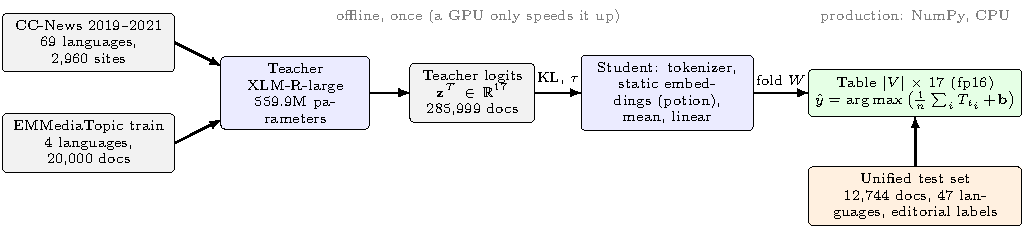
\includegraphics[width=\textwidth]{figures/fig_pipeline.pdf}
\caption{StaticKD pipeline from one-time teacher labeling to inference with the folded token table.}
\label{fig:pipeline}
\end{figure*}

\subsection{Problem Formulation}
A model predicts one label $y\in\mathcal{Y}$ among the 17 top-level IPTC topics for a news article $d$ in any language. The input is the title and body truncated to the first 512 words as in~\cite{kuzman2025llm}. Each model then applies its own token limit to this input (Sections~\ref{sec:teacher} and~\ref{sec:student}). The teacher $f_T$ outputs logits $\mathbf{z}^T(d)\in\mathbb{R}^{17}$ for this input. The study seeks a student $f_S$ whose accuracy against independent labels is as close as possible to that of $f_T$. Inference with $f_S$ is restricted to $O(n)$ additions for $n$ tokens and uses neither matrix multiplication nor a deep learning library.

\subsection{Teacher and Distillation Labels}
\label{sec:teacher}
The teacher is the IPTC classifier of~\cite{kuzman2025llm} published as \url{classla/multilingual-IPTC-news-topic-classifier}. It is an XLM-RoBERTa-large model with 24 layers, 559.9 million parameters, and an input limit of 512 XLM-R tokens. The teacher labeled all distillation data at a one-time cost of about 1.6 GPU hours and produced the full logit vector $\mathbf{z}^{T}(d)\in\mathbb{R}^{17}$ that was stored for every distillation document.

\subsection{The StaticKD Student}
\label{sec:student}
The student is built on the multilingual static embedding model potion-multilingual-128M (potion) of Model2Vec~\cite{tulkens2024model2vec}. The embedding matrix $E$ of the student is initialized from potion so that the tokens of 101 languages lie in one shared space before training starts. A document $d$ is tokenized into $t_1,\dots,t_n$ with the 500,353-token Unigram tokenizer of potion so that every token has a pre-trained embedding. Special tokens are not used and unknown tokens are dropped. Averaging ignores token position and gives the model no built-in length limit. Document length is capped at 1,024 tokens to bound the cost. Only 5.4\% of the test articles exceed this cap. The student computes the document logits from the average of the token embeddings $\mathbf{e}_t\in\mathbb{R}^{256}$:
\begin{equation}
\mathbf{h}(d)=\frac{1}{n}\sum_{i=1}^{n}\mathbf{e}_{t_i},\qquad
\mathbf{z}^{S}(d)=W\,\mathrm{drop}(\mathbf{h}(d))+\mathbf{b},
\label{eq:student}
\end{equation}
with $W\in\mathbb{R}^{17\times 256}$ and dropout 0.1 on $\mathbf{h}(d)$ during training.

The student learns from the stored teacher logits with the loss
\begin{equation}
\mathcal{L}_{\mathrm{KD}}=\tau^{2}\,\mathrm{KL}\!\left(p^{T}\,\middle\|\,p^{S}\right),\qquad \tau=1 ,
\label{eq:kd}
\end{equation}
where $p^{T}=\mathrm{softmax}(\mathbf{z}^{T}/\tau)$ and $p^{S}=\mathrm{softmax}(\mathbf{z}^{S}/\tau)$ are the teacher and student distributions. The value $\tau=1$ was fixed together with the other recipe choices (Section~\ref{sec:roles}) and the results for the other values $\tau\in\{0.5,2,4\}$ are reported in Section~\ref{sec:res-abl}. The parameters $E$, $W$, and $\mathbf{b}$ are trained together. AdamW ($\eta=3\cdot 10^{-3}$, weight decay $10^{-4}$) updates $W$ and $\mathbf{b}$ whereas SparseAdam ($\eta=10^{-3}$) updates the embedding matrix $E$ only in the rows of tokens that occur in the current batch. Tokens that never occur in the training documents therefore keep the potion embeddings. Training runs for 6 epochs with a batch size of 64. Token dropout is a cheap augmentation that drops each token of a training document with probability 0.2 at every step so that the model does not rely on a few keywords. This augmentation differs from the dropout of 0.1 on $\mathbf{h}(d)$ in Eq.~\eqref{eq:student}. Internal validation uses 3\% of the distillation data (8,579 documents) to keep the epoch with the highest agreement with the teacher.

\subsection{Folding, Table Ensemble, and Compact Variant}
\label{sec:fold}
The linear classification head allows \eqref{eq:student} to be rewritten as
\begin{equation}
W\Big(\frac{1}{n}\sum_{i}\mathbf{e}_{t_i}\Big)+\mathbf{b}=\frac{1}{n}\sum_{i}T_{t_i}+\mathbf{b},
\label{eq:fold}
\end{equation}
with the table $T=EW^{\top}\in\mathbb{R}^{|V|\times 17}$ computed once after training in the folding step. Row $T_t$ of the table $T$ holds the 17 topic scores that token $t$ contributes to every article that contains it. Fig.~\ref{fig:folding} shows that the 256-dimensional matrix $E$ is needed only during training so that the folded model for deployment consists of $T$ in half precision (fp16), $\mathbf{b}$, and the tokenizer. The same folding argument holds for an ensemble because Eq.~\eqref{eq:fold} is linear in $T$. Averaging the logits of $K$ students trained with different seeds gives the same result as one student with table $\bar{T}=\frac{1}{K}\sum_k T^{(k)}$ and bias $\bar{\mathbf{b}}$.

\begin{figure*}[!t]
\centering
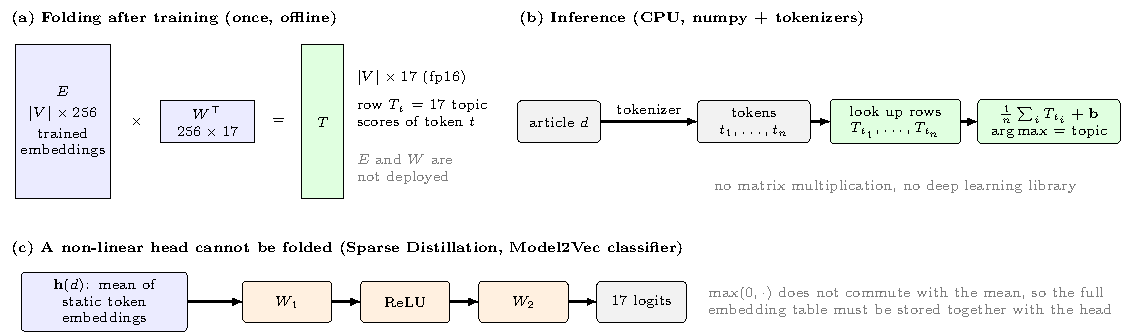
\includegraphics[width=\textwidth]{figures/fig_folding.pdf}
\caption{Folding of the embeddings $E$ and the linear head $W$ into the token table $T$.}
\label{fig:folding}
\end{figure*}

The final StaticKD model averages the tables of three students ($K=3$) and has 8.5 million parameters. The model file is 34~MB in size and the averaged table accounts for 16~MB of it. Most of the random-access memory (RAM) that the model uses during inference goes to the internal structure of the Unigram tokenizer. The compact variant shrinks this structure by removing token pieces that occur fewer than 10 times in the distillation data but keeps single characters. Its vocabulary holds 335,441 tokens and its file is 23~MB in size.

\section{Data and Test Set}
\label{sec:data}
\subsection{Data Sets and Their Roles}
\label{sec:roles}
Table~\ref{tab:datasets} shows that the development set and the internal validation used to choose the model settings are separate from the unified test set. A development set is a labeled data set used to choose the model settings before the final measurement so that the test set does not influence these choices. The development set of this study is the development split of EMMediaTopic (Section~\ref{sec:distdata}). The parameter settings and recipe choices of StaticKD were fixed before the test set was built. The development set was also used to test four additional components: bigram features, idf-weighted pooling, document weighting by teacher confidence, and an auxiliary loss on the GPT-4o labels. None of the four entered the recipe because none of them changed the development set score significantly.

\begin{table}[!t]
\caption{Data Sets of the Study and Their Roles}
\label{tab:datasets}
\centering
\footnotesize
\setlength{\tabcolsep}{3pt}
\resizebox{\columnwidth}{!}{%
\begin{tabular}{@{}lrrll@{}}
\toprule
Set & Docs & Lang. & Labels & Used for \\
\midrule
Distillation data & 285,999 & 69 & teacher & training the students \\
\quad internal validation & 8,579 & -- & teacher & choosing the epoch \\
Development (EMMediaTopic) & 1,000 & 4 & GPT-4o & choosing the recipe \\
CC-News held-out & 12,554 & 63 & teacher & agreement, unseen sites \\
Unified test set & 12,744 & 47 & human, editorial & all accuracy results \\
English section sample & 754 & 1 & JSON-LD & label validity only \\
\bottomrule
\end{tabular}}
\end{table}

\subsection{Distillation Data and Development Set}
\label{sec:distdata}
The development set and part of the distillation data come from EMMediaTopic 1.0~\cite{emmediatopic2025,kuzman2025llm}. EMMediaTopic contains GPT-4o-labeled articles in four languages (Catalan, Greek, Croatian, and Slovenian). A total of 21,000 annotated articles were taken and divided into a training split of 20,000 and a development split of 1,000 articles. Kuzman and Ljube\v{s}i\'c trained the teacher on the training split and tuned its hyperparameters on the development split~\cite{kuzman2025llm}. The training split also forms part of the distillation data for the student. Neither the teacher nor the student was ever trained on the development split.

Most of the distillation data come from the multilingual CC-News 2019--2021 dataset~\cite{cloversearch_ccnews} built from the news archive of Common Crawl. CC-News 2019--2021 was processed with the following steps.
\begin{enumerate}
  \item Verify the language with the fastText language identification model~\cite{joulin2017bag} and keep only documents whose metadata language agrees with the identified language.
  \item Keep documents whose title and body reach 75 words in total and truncate the text to 512 words. Documents in Japanese, Chinese, Thai, and Burmese use limits of 200 and 2,000 characters instead.
  \item Set aside all documents of some sites as a held-out set that is not used for training and holds at most 20\% of each language.
  \item Cap the number of training documents per site to avoid bias from similar content within one site.
\end{enumerate}
The final distillation data contain 285,999 documents in 69 languages from 2,960 sites with a median document length of 269 words and at most 400 documents per site. They consist of a base version of about 130 thousand documents with at most 150 documents per site and 156,157 additional documents from training sites only (at most 5,000 per language). The base version is also used as an ablation variant (Section~\ref{sec:design}).

The held-out set contains 12,554 documents in 63 languages from 217 sites that never occur in the distillation data. It can only measure agreement with the teacher because it has no independent category labels.

\subsection{Unified Test Set Construction}
\label{sec:testset}
The largest source of the unified test set is the CC-NEWS 2024--2026 dataset~\cite{commoncrawl2026ccnews} sampled as one archive file (WARC) per month from January 2024 to August 2026 (32 files). Each article page carries structured schema.org metadata~\cite{guha2016schema} in JSON-LD format that provides the article section and other metadata in fields such as \texttt{articleSection}, \texttt{BreadcrumbList}, \texttt{inLanguage}, \texttt{datePublished}, \texttt{isAccessibleForFree}, and \texttt{articleBody}. The text was taken from \texttt{articleBody} only when that field had at least 30 words. Trafilatura~\cite{barbaresi2021trafilatura} extracted the text of other articles from the HTML content.

All other test articles come from the five public datasets of Section~\ref{sec:rw-iptc}. L3Cube-IndicNews articles were taken from the LDC split of long documents. The publisher categories of these datasets and the JSON-LD sections both count as editorial labels.

Section names have to be translated onto the official IPTC Media Topic tree (1,085 active nodes) because editorial labels do not follow the IPTC standard. The section names were first normalized for case and diacritics and then mapped conservatively by an LLM (Claude Opus 5.5). The LLM read the section names without the article texts and mapped a name only if the subject that the name states falls under a single top-level topic of the IPTC tree. An automatic check verified that every target node exists in the IPTC tree, is still active, and lies under the intended top-level topic. The mapping table drafted by the LLM was then evaluated and corrected manually by human reviewers. The final table links 814 section names to 79 IPTC nodes. Articles whose sections in the \texttt{articleSection} and \texttt{BreadcrumbList} fields mapped to different labels were rejected so that every article has one label.

Quality and leakage filters were applied in order.
\begin{enumerate}
  \item Site absent from both the distillation data and the held-out set (CC-NEWS only).
  \item Publication date on or after 1 January 2024 (CC-NEWS only).
  \item Full article text and not a teaser.
  \item Declared language agrees with fastText language identification when fastText supports the language.
  \item At least 75 words.
  \item Deduplication of uniform resource locators (URLs), identical texts, and near-duplicates (MinHash~\cite{broder1997resemblance}, Jaccard $\ge 0.7$~\cite{lee2022dedup}) across all sources.
  \item Contamination: an article was dropped when $\ge 30\%$ of its word 8-grams occurred in any of about 300 thousand training or evaluation documents.
\end{enumerate}

Sampling of the articles that passed all filters took at most 50 articles for each pair of language and label and gave priority to human-labeled sources. The final test set contains 12,744 articles in 47 languages from 1,227 sites or sources with a median article length of 313 words. All 17 labels occur in this test set although the articles of one language cover a median of 7 of the 17 labels. The \emph{label origin} of an article is human annotation for 4,094 articles (32.1\%), publisher category for 2,600 articles (20.4\%), and JSON-LD section for 6,050 articles (47.5\%). Table~\ref{tab:testset} shows that the publisher diversity comes mainly from CC-NEWS with its 1,092 sites in 29 languages.

\begin{figure*}[!t]
\centering
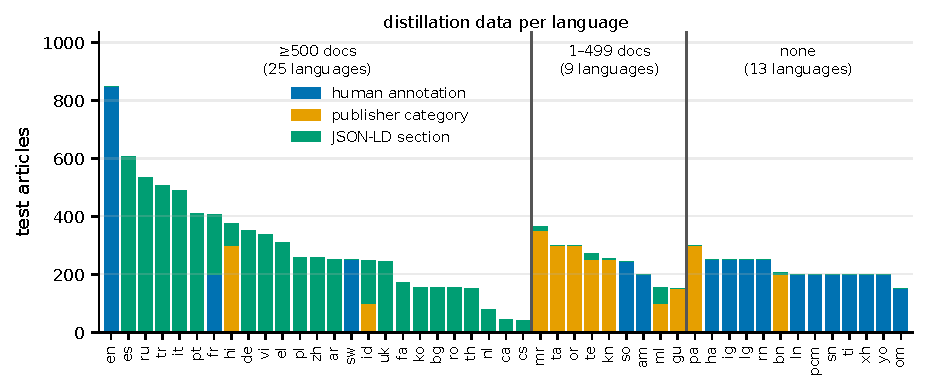
\includegraphics[width=\textwidth]{figures/fig_testset_composition.pdf}
\caption{Unified test set articles per language by label origin and amount of distillation data.}
\label{fig:testset}
\end{figure*}

The amount of distillation data differs across the test set languages and is used for the subgroup analysis (Section~\ref{sec:protocol}). No distillation data exist for 13 languages whereas 9 other languages have fewer than 500 distillation documents and the remaining 25 languages have at least 500. Fig.~\ref{fig:testset} shows that the labels of languages with no or little distillation data come almost entirely from human annotation or publisher categories whereas JSON-LD sections mainly cover languages with at least 500 distillation documents.

\begin{table}[!t]
\caption{Composition of the Unified Test Set by Source}
\label{tab:testset}
\centering
\footnotesize
\setlength{\tabcolsep}{3pt}
\resizebox{\columnwidth}{!}{%
\begin{tabular}{@{}llrrr@{}}
\toprule
Source & Label origin & Articles & Languages & Sites/sources \\
\midrule
CC-NEWS 2024--2026 & JSON-LD section & 6,050 & 29 & 1,092 \\
MasakhaNEWS~\cite{adelani2023masakhanews} & human annotation & 3,339 & 16 & 6 \\
L3Cube-IndicNews~\cite{mirashi2023indicnews} & publisher category & 2,361 & 10 & 1 \\
MN-DS~\cite{petukhova2023mnds} & human annotation & 755 & 1 & 127 \\
Bangla news~\cite{hossain2025banglanews} & publisher category & 139 & 1 & 1 \\
IndoNews & publisher category & 100 & 1 & 1 \\
\midrule
Total & & 12,744 & 47 & 1,227 \\
\bottomrule
\end{tabular}}
\par\vspace{2pt}{\footnotesize One site (jpost.com) occurs in both CC-NEWS and MN-DS so the site total is one less than the column sum.\par}
\end{table}

\subsection{Label Validity Check}
\label{sec:validity-design}
Two thirds of the test labels are section and category labels that record newsroom decisions rather than annotation that follows a labeling guideline. The label validity check tests whether such labels behave like human labels in the same language (Section~\ref{sec:res-validity}). The teacher is a fixed reference for both label types and would agree less often with section labels than with human labels if the section labels carried much more noise. This agreement is measured with the accuracy and macro-F1 of the teacher on each label type, a Wilcoxon signed-rank test on the per-label accuracies, and the Spearman correlation between the label difficulty rankings of the two label types. A per-category analysis also checks the mapping by comparing the predictions of the teacher with the mapped label of each source category in languages covered by XLM-R pre-training.

A comparison between label types needs section labels and human labels in the same language. The test set itself provides section labels and the human labels of MasakhaNEWS in French. The English part of the test set contains only human labels because the sampling preferred human-labeled sources (Section~\ref{sec:testset}). A comparison within English has to use a sample of articles that are not in the test set. This sample contains 754 English CC-NEWS articles from 306 sites with JSON-LD section labels and at most 50 articles per label.

\section{Experimental Setup}
\label{sec:setup}
\subsection{Baselines}
\label{sec:baselines}
All baselines marked + KD used the same distillation data (285,999 documents) and targets from the same teacher. Table~\ref{tab:baselines} shows that only the two transformer baselines learn from the full teacher distribution. The three light baselines were trained on the top teacher label because their standard training procedures accept class labels but not probability distributions. The light baselines are fastText + KD~\cite{joulin2017bag}, term frequency--inverse document frequency (TF-IDF) + support vector machine (SVM) + KD, and the Model2Vec classifier + KD~\cite{tulkens2024model2vec}. TF-IDF + SVM + KD adapts the non-neural baseline of Kuzman and Ljube\v{s}i\'c to the teacher labels. The Model2Vec classifier + KD fine-tunes the same potion embeddings that StaticKD starts from and learns a weight for each token. Two further fastText models were trained only on the GPT-4o labels of the EMMediaTopic training split as a reference without KD that uses the same labeled data as the teacher~\cite{kuzman2025llm}.

MiniLM-L6 + KD and DistilmBERT + KD are transformer baselines trained with the loss in~\eqref{eq:kd} on the full teacher distribution. MiniLM-L6 + KD uses mMiniLMv2-L6-H384 distilled from XLM-R-large~\cite{wang2021minilmv2} whereas DistilmBERT + KD uses \texttt{distilbert-base-multilingual-cased}~\cite{sanh2019distilbert}. The 256-token limit truncates 91.1\% of the test articles to about 142 words for MiniLM-L6 and 93.2\% to about 116 words for DistilmBERT. A sensitivity check of this limit retrained both models with 512 tokens (Section~\ref{sec:res-acc}).

Sparse Distillation~\cite{ye2022sparse} is the prior method closest to StaticKD but was not run as a separate baseline (Section~\ref{sec:limitations}). Two other experiments still cover parts of the method. The fastText + KD baseline trained a bag-of-n-grams model with averaging and a linear head on the same teacher labels. The random-initialization ablation (Section~\ref{sec:design}) trained the embedding table from scratch as Sparse Distillation does.

\begin{table*}[!t]
\caption{Baselines and Their Training}
\label{tab:baselines}
\centering
\footnotesize
\setlength{\tabcolsep}{4pt}
\resizebox{\textwidth}{!}{%
\begin{tabular}{@{}llll@{}}
\toprule
Model & Inference-time representation & Training target & Tuning \\
\midrule
fastText + KD, word & mean of word and character n-gram vectors, linear head & top teacher label & grid search on development set \\
fastText + KD, subword & mean of XLM-R subword vectors, linear head & top teacher label & grid search on development set \\
fastText + KD, subword, quantized & subword variant in \texttt{.ftz} format & top teacher label & from subword variant \\
TF-IDF + SVM + KD & TF-IDF over XLM-R subwords, linear SVM & top teacher label & grid search on development set \\
Model2Vec classifier + KD & fine-tuned potion embeddings with per-token weights, hidden layer of 512 units & top teacher label & library default settings \\
MiniLM-L6 + KD & 6-layer transformer, 256-token input & full teacher distribution & $\tau\in\{1,2\}$ on development set \\
DistilmBERT + KD & 6-layer transformer, 256-token input & full teacher distribution & $\tau=1$ \\
fastText, GPT-4o labels (word, subword) & as fastText + KD & EMMediaTopic GPT-4o labels & fixed settings \\
\bottomrule
\end{tabular}}
\end{table*}

\subsection{Evaluation Protocol and Statistical Tests}
\label{sec:protocol}
Table~\ref{tab:protocol} lists macro-F1 as the main metric because the label distribution is imbalanced. The metric is the unweighted mean of F1 over the labels present in the reference as in the evaluation protocol of~\cite{kuzman2025llm}. The per-language macro-F1 is averaged over languages so that large languages do not dominate. Calibration was measured with the expected calibration error (ECE)~\cite{guo2017calibration} because the cascade mode in Section~\ref{sec:effprotocol} routes articles by the confidence of StaticKD.

Confidence intervals and paired tests use a bootstrap with a different resampling unit on each of the two evaluation sets. The development set was resampled by document whereas the test set used a site-cluster bootstrap~\cite{field2007bootstrapping} that draws whole sites as the resampling unit so that related articles from one site do not make the confidence intervals too narrow. Articles without a URL are grouped by source dataset.

Two additional checks test the robustness of the model comparison because the clusters of the test set differ in size. The two largest of the 1,227 clusters (bbc.com and L3Cube-IndicNews) hold 37.3\% of the articles and the effective number of clusters $1/\sum_c q_c^{2}$ with $q_c$ as the share of cluster $c$ is 13.8. A leave-one-source-out check recomputed the macro-F1 of the teacher and StaticKD together with the seven + KD baselines once without each of the six test-set sources. Another check repeated the model comparison on a subset with at most five articles per site and language--label pair.

Claims of equivalence rest on two one-sided tests (TOST) over the same bootstrap distribution because a difference that is not significant in a paired test does not show that two models are equivalent. The margin of 0.01 macro-F1 was treated as a negligible difference for topic filtering. Holm correction was applied separately on the development set and the test set over all comparisons of StaticKD with other models in Table~\ref{tab:sig}.

The same paired bootstrap compared each ablation variant with the final recipe. Every resample scored all seeds of the variant and of the final recipe on the same articles and yielded the difference between the two seed means as the tested quantity. The score of an ensemble of $K$ students is the mean score over all combinations of $K$ of the ten final-recipe seeds. Holm correction for these comparisons covered the 10 variants of Section~\ref{sec:design} and the four additional components of Section~\ref{sec:roles} with three seeds each.

The per-language analysis used two quantities. The \emph{accuracy gap} is the StaticKD accuracy minus the teacher accuracy. The \emph{token coverage} of a language is the share of all token occurrences in its test articles whose token occurs at least 10 times in the distillation data. This threshold was used because training seldom updates the embeddings of less frequent tokens (Section~\ref{sec:student}).

Subgroup analyses split the results by language, script, region, label, label origin, site diversity, amount of distillation data per language, and teacher pre-training coverage. The site diversity of a language is measured by the effective number of sites $1/\sum_s q_s^{2}$ with $q_s$ as the share of the articles of that language that come from site $s$. Pre-training coverage refers to whether the language is among the 100 languages used to pre-train XLM-R~\cite{conneau2020xlmr}.

Seven tests with jointly Holm-corrected $p$-values checked whether the properties of a language explain the performance of StaticKD on that language. Four tests examined the similarity of StaticKD to the teacher on the 53 languages with at least 20 held-out documents. Three of them were Spearman correlations of held-out agreement with the log amount of distillation data, the number of training sites, and the teacher confidence whereas a Kruskal--Wallis test compared agreement across scripts. The other three tests examined how far StaticKD falls behind the teacher on the test set through Spearman correlations between the accuracy gap and the log amount of distillation data, between StaticKD accuracy and token coverage, and between the accuracy gap and token coverage.

The token-table analysis measures the \emph{specificity} of a token as the largest difference between one entry of its table row and the mean of the other 16 entries. A pruning test kept only the 10\% most specific tokens of each article and compared the result with that of a random 10\% of the tokens to measure how much topic signal the most specific tokens carry.

\begin{table}[!t]
\caption{Summary of the Evaluation Protocol and Statistical Tests}
\label{tab:protocol}
\centering
\footnotesize
\setlength{\tabcolsep}{3pt}
\begin{tabular}{@{}p{0.30\columnwidth}p{0.66\columnwidth}@{}}
\toprule
Question & Metric or test \\
\midrule
Accuracy against independent labels & macro-F1 (main), accuracy, and per-language macro-F1 \\
Similarity to the teacher & agreement on the held-out set \\
Calibration & ECE with 15 bins \\
Score uncertainty & 95\% confidence interval from a percentile bootstrap with 1,000 resamples \\
Difference between two models & paired bootstrap with 2,000 resamples for $\Delta$macro-F1~\cite{koehn2004significance}, exact McNemar for accuracy~\cite{mcnemar1947}, and Holm correction~\cite{holm1979} \\
Equivalence of two models & TOST~\cite{schuirmann1987tost} with the 90\% interval within $\pm$0.01 \\
Consistency across languages & Wilcoxon signed-rank on per-language macro-F1 and accuracy~\cite{dror2018hitchhiker} \\
Effect of recipe components & ablation with five seeds per variant and ten seeds for the final recipe \\
Language properties & six Spearman correlations and one Kruskal--Wallis test with joint Holm correction \\
Robustness to clusters & leave-one-source-out and a subset with at most five articles per site and language--label pair \\
\bottomrule
\end{tabular}
\end{table}

\subsection{Efficiency Protocol}
\label{sec:effprotocol}
Table~\ref{tab:effsetup} shows that all models were measured with the same setup so that the speed ratios between models are comparable. The CPU of the laptop is hybrid and has 6 performance cores (P-cores), 8 slower efficiency cores (E-cores), and 2 low-power E-cores. Each process was pinned to physical P-cores because the operating system moves unpinned threads to the slow cores. The pinned setup approximates a small server with uniform cores. The single-core throughput of every model deviated by at most 7\% from the median of the three measurement sessions. A separate single-thread profile split the prediction time of StaticKD into tokenization time and table-averaging time on 1,280 articles to find the step that limits its speed.

Both transformer baselines were exported to the Open Neural Network Exchange (ONNX) format in fp32 for the CPU benchmark. The teacher was also exported to ONNX with dynamic quantization to 8-bit integers (int8). The ONNX int8 teacher is the fastest teacher configuration on CPU.

\begin{table}[!t]
\caption{CPU Benchmark Setup}
\label{tab:effsetup}
\centering
\footnotesize
\setlength{\tabcolsep}{3pt}
\begin{tabular}{@{}p{0.22\columnwidth}p{0.74\columnwidth}@{}}
\toprule
Aspect & Setting \\
\midrule
Machine & Intel Core Ultra~7 155H laptop, 32~GB RAM, Windows~11, GPU disabled \\
Process & fresh process per model, thread count pinned in every library, one or four physical P-cores \\
Sample & same random text sample from the unified test set \\
Latency & median (p50) and 95th percentile (p95) with one article per call (streaming scenario); 100 documents for teacher and transformers, 500 documents for light models \\
Throughput & batch 64 (8 for transformers); 96 documents for teacher and transformers, 3,000 documents for light models \\
Model RAM & increase in resident set size after the model is loaded \\
Repetition & three sessions on an idle machine, median reported \\
\bottomrule
\end{tabular}
\end{table}

The speed comparison does not favor StaticKD because StaticKD reads longer inputs. StaticKD reads up to 1,024 tokens per article whereas the teacher stops at 512 XLM-R tokens. The teacher limit is exceeded by 60.7\% of the test-set articles and on these articles the teacher reads about 287 of 438 words (median).

The cascade mode combines StaticKD and the teacher for workloads that need teacher-level accuracy. The mode lets StaticKD decide the articles on which its top probability is at least a threshold $\theta$ and passes the remaining articles to the ONNX int8 teacher. Let $s$ be the share of articles decided by StaticKD and let $r_S$ and $r_T$ be the single-core throughputs of StaticKD and the teacher. The effective throughput of the cascade is $1/(1/r_S+(1-s)/r_T)$.

\subsection{Ablation Design}
\label{sec:design}
Each ablation variant changes one factor of the final recipe. One variant replaces the soft labels with hard labels and two variants reduce the training data either to EMMediaTopic only (4 languages, 10 epochs) or to 130 thousand documents without the extra CC-News 2019--2021 data. Other variants freeze the embeddings or draw random embeddings with the same standard deviation as potion. The remaining variants train without token dropout, use a 512-unit MLP head, or set $\tau\in\{0.5,\,2,\,4\}$. Table~\ref{tab:ablation} lists the final recipe and all of these variants.

\subsection{Implementation Details}
\label{sec:impl}
An average StaticKD run took 5.2 minutes on an NVIDIA RTX~4050 Laptop GPU. The implementation uses Python~3.12, NumPy~2.5, PyTorch~2.6, transformers~5.17, \texttt{tokenizers}~0.23, ONNX Runtime~1.30, scikit-learn~1.9, and fastText~0.9.2.

\section{Results}
\label{sec:results}
\subsection{Validity of the Editorial Labels}
\label{sec:res-validity}
The agreement of the teacher with both label types shows that English section labels are not noisier than human labels. The teacher reaches an accuracy of 0.646 on the 754 English articles with section labels (macro-F1 0.617) and 0.559 on the English human labels of MN-DS and MasakhaNEWS (macro-F1 0.565). Teacher accuracy is higher on the section labels for 12 of the 17 labels (Wilcoxon $p=0.033$). Label difficulty rankings also correlate between the two label types ($\rho=0.63$, $p=0.007$) and both label types share the same difficult labels \emph{society}, \emph{human interest}, and \emph{religion}. French data in the test set also contain both label types. The teacher is again more accurate on section labels there (0.716 on 208 articles against 0.500 on 200 human-labeled MasakhaNEWS articles).

The per-category agreement between the teacher and the mapped label is lowest for source categories that are broader than the IPTC target and for labels with unclear boundaries. Median agreement per category is higher for L3Cube (0.81) and CC-NEWS sections (0.87) than for MasakhaNEWS (0.46) and MN-DS (0.50). Articles in the \emph{politics} category of MasakhaNEWS are predicted as \emph{politics} in 45\% of cases and as \emph{conflict} in 29\%. The \emph{society} label of MN-DS is an example of a label with unclear boundaries.

\subsection{Accuracy of All Models}
\label{sec:res-acc}
\begin{table*}[!t]
\caption{Main Results on the Development, Held-Out, and Unified Test Sets}
\label{tab:main}
\centering
\scriptsize
\setlength{\tabcolsep}{3.5pt}
\begin{tabular}{@{}lccccccc@{}}
\toprule
 & \multicolumn{2}{c}{dev (4 languages)} & held-out & \multicolumn{4}{c}{unified test (47 languages)} \\
\cmidrule(lr){2-3}\cmidrule(lr){4-4}\cmidrule(lr){5-8}
Model & Macro-F1 [95\% CI] & Accuracy & Agreement & Macro-F1 [95\% CI] & Accuracy & Macro-F1/language & \% teacher \\
\midrule
Teacher XLM-R-large & 0.822 [0.779--0.851] & 0.859 & -- & 0.598 [0.546--0.643] & 0.700 & 0.705 & 100.0\% \\
Teacher XLM-R-large, ONNX int8 & 0.823 [0.781--0.852] & 0.858 & -- & 0.600 [0.547--0.646] & 0.699 & 0.702 & 100.3\% \\
\midrule
DistilmBERT + KD & 0.753 [0.710--0.785] & 0.801 & 0.799 & 0.534 [0.481--0.618] & 0.623 & 0.602 & 89.4\% \\
MiniLM-L6 + KD & 0.785 [0.737--0.815] & 0.820 & 0.825 & 0.566 [0.511--0.624] & 0.667 & 0.661 & 94.6\% \\
\midrule
\textbf{StaticKD (proposed)} & \textbf{0.761 [0.717--0.792]} & 0.800 & 0.811 & \textbf{0.545 [0.490--0.605]} & 0.641 & 0.622 & 91.1\% \\
StaticKD-compact & 0.754 [0.710--0.786] & 0.797 & 0.802 & 0.484 [0.421--0.597] & 0.544 & 0.507 & 81.0\% \\
\midrule
fastText + KD, subword, quantized & 0.729 [0.688--0.760] & 0.768 & 0.740 & 0.439 [0.370--0.561] & 0.515 & 0.465 & 73.4\% \\
fastText + KD, subword & 0.737 [0.701--0.765] & 0.772 & 0.754 & 0.447 [0.385--0.566] & 0.527 & 0.480 & 74.7\% \\
fastText + KD, word & 0.750 [0.713--0.779] & 0.791 & 0.758 & 0.445 [0.380--0.563] & 0.515 & 0.474 & 74.5\% \\
TF-IDF + SVM + KD & 0.755 [0.719--0.786] & 0.798 & 0.776 & 0.486 [0.431--0.585] & 0.567 & 0.522 & 81.3\% \\
Model2Vec classifier + KD & 0.744 [0.701--0.772] & 0.780 & 0.805 & 0.547 [0.495--0.599] & 0.642 & 0.619 & 91.5\% \\
\midrule
fastText, GPT-4o labels, subword & 0.665 [0.613--0.700] & 0.729 & 0.260 & 0.086 [0.069--0.119] & 0.150 & 0.118 & 14.4\% \\
fastText, GPT-4o labels, word & 0.651 [0.601--0.693] & 0.738 & 0.307 & 0.106 [0.085--0.150] & 0.181 & 0.142 & 17.7\% \\
\bottomrule
\end{tabular}
\end{table*}
Table~\ref{tab:main} shows that StaticKD keeps 91.1\% of the teacher macro-F1 on the unified test set and 92.6\% on the development set. The test macro-F1 is 0.545 [0.490--0.605] for StaticKD and 0.598 [0.546--0.643] for the teacher. The test scores of both models are lower than their development scores (0.761 and 0.822) because most of the test set lies outside the languages, sources, and period of the teacher training data. StaticKD agrees with the teacher on 81.1\% of the held-out documents in 63 languages.

The test macro-F1 of StaticKD lies between the scores of the two distilled transformers and above those of fastText + KD and TF-IDF + SVM + KD. MiniLM-L6 (0.566) is ahead of StaticKD whereas DistilmBERT (0.534) is slightly behind. The Model2Vec classifier reaches 0.547 and scores almost the same as StaticKD. The fastText model trained only on the GPT-4o labels of four languages shows what happens when there are no teacher labels for other languages (last two rows of Table~\ref{tab:main}). This model reaches 0.665 on the development set but only 0.086 on the test set.

\begin{table*}[!t]
\caption{Paired Tests of StaticKD Against Other Models on the Unified Test Set}
\label{tab:sig}
\centering
\scriptsize
\begin{tabular}{@{}lccccc@{}}
\toprule
StaticKD vs & $\Delta$macro-F1 [95\% CI] & $p$ bootstrap & $\Delta$accuracy & McNemar $b/c$ & $p$ McNemar \\
\midrule
Teacher XLM-R-large & $-$0.053 [$-$0.065, $-$0.033] & $<$0.001 & $-$0.059 & 654/1400 & $<$0.001 \\
Teacher XLM-R-large, ONNX int8 & $-$0.055 [$-$0.067, $-$0.035] & $<$0.001 & $-$0.058 & 644/1386 & $<$0.001 \\
DistilmBERT + KD & +0.010 [$-$0.026, +0.041] & 1.000 & +0.018 & 1372/1143 & $<$0.001 \\
MiniLM-L6 + KD & $-$0.021 [$-$0.038, $-$0.008] & 0.005 & $-$0.026 & 866/1197 & $<$0.001 \\
StaticKD-compact & +0.060 [+0.003, +0.100] & 0.042 & +0.097 & 1345/110 & $<$0.001 \\
fastText + KD, subword, quantized & +0.106 [+0.037, +0.145] & $<$0.001 & +0.126 & 2135/532 & $<$0.001 \\
fastText + KD, subword & +0.098 [+0.036, +0.134] & $<$0.001 & +0.114 & 1979/529 & $<$0.001 \\
fastText + KD, word & +0.099 [+0.037, +0.141] & $<$0.001 & +0.126 & 2140/536 & $<$0.001 \\
TF-IDF + SVM + KD & +0.059 [+0.009, +0.093] & 0.040 & +0.074 & 1667/719 & $<$0.001 \\
Model2Vec classifier + KD & $-$0.002 [$-$0.009, +0.010] & 1.000 & $-$0.001 & 438/447 & 0.788 \\
fastText, GPT-4o labels, subword & +0.458 [+0.415, +0.496] & $<$0.001 & +0.491 & 6597/344 & $<$0.001 \\
fastText, GPT-4o labels, word & +0.439 [+0.393, +0.475] & $<$0.001 & +0.460 & 6252/391 & $<$0.001 \\
\bottomrule
\end{tabular}
\par\vspace{2pt}{\footnotesize $\Delta$ = StaticKD $-$ comparison model; $b/c$ = documents correct only for StaticKD / only for the comparison model.\par}
\end{table*}
\begin{figure}[!t]
\centering
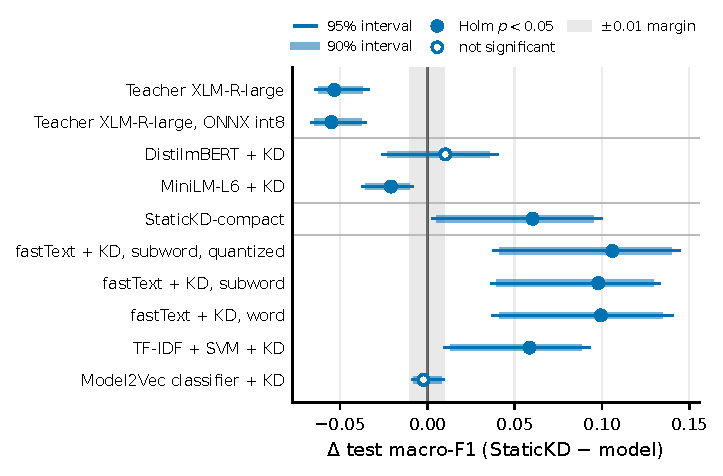
\includegraphics[width=\columnwidth]{figures/fig_sig_forest.pdf}
\caption{Paired difference in test macro-F1 between StaticKD and each model except the two fastText models trained on GPT-4o labels.}
\label{fig:sig-forest}
\end{figure}
The paired tests in Table~\ref{tab:sig} confirm this ranking. Fig.~\ref{fig:sig-forest} shows that the 95\% intervals of the differences between StaticKD and all light models except the Model2Vec classifier lie above zero whereas the intervals against the teacher and MiniLM-L6 lie below zero. The $\Delta$macro-F1 of StaticKD against the teacher is $-$0.053 [$-$0.065, $-$0.033] and StaticKD beats the teacher in only 7 of 47 languages. MiniLM-L6 also keeps a significant lead over StaticKD ($-$0.021 [$-$0.038, $-$0.008], $p=0.005$). StaticKD and DistilmBERT do not differ significantly (+0.010, $p=1.000$) and the 90\% interval [$-$0.023, +0.036] of this difference is too wide to show equivalence (TOST $p=0.428$). The per-language Wilcoxon test also finds no consistent difference between the two models ($p=0.604$ for macro-F1 and 0.322 for accuracy). The McNemar test favors StaticKD over DistilmBERT in accuracy ($p<0.001$) but treats articles from the same site as independent.

The Model2Vec classifier is the only light model that matches StaticKD. The $\Delta$macro-F1 between the two models is $-$0.002 [$-$0.009, +0.010] with a 90\% interval of [$-$0.008, +0.008] inside the $\pm$0.01 equivalence margin (TOST $p=0.025$). The per-language comparison with the Model2Vec classifier also shows no consistent difference in either metric (Wilcoxon $p=0.358$ for macro-F1 and 0.534 for accuracy).

StaticKD is ahead of the quantized fastText + KD by +0.106 [+0.037, +0.145] and of TF-IDF + SVM by +0.059 [+0.009, +0.093] ($p=0.040$). The macro-F1 of StaticKD is higher than that of fastText + KD in 40 of 47 languages (Wilcoxon $p<0.001$). The advantage over TF-IDF + SVM is narrower with a higher StaticKD macro-F1 in 31 of 47 languages (Wilcoxon $p=0.003$). Per-language accuracy against TF-IDF + SVM gives a different picture because StaticKD is higher in 24 languages and lower in 22 (Wilcoxon $p=0.127$).

The model ranking hardly changes when checked against the cluster structure of the test set. The subset with at most five articles per site and language--label pair keeps 8,139 articles with a score of 0.587 for StaticKD and 0.627 for the teacher. Only the order of StaticKD and the Model2Vec classifier (0.583) changes on this subset. Leaving out one source at a time places StaticKD between third and fifth of the nine models and only the Model2Vec classifier and DistilmBERT change places with it. Every fastText and TF-IDF model stays at least 0.028 below StaticKD.

Paired test results also stay the same when the two transformers read longer inputs. Retraining with 512-token inputs raises the test macro-F1 of MiniLM-L6 and DistilmBERT to 0.580 and 0.547. MiniLM-L6 stays ahead of StaticKD ($-$0.035 [$-$0.049, $-$0.021], $p<0.001$) and DistilmBERT still does not differ significantly from StaticKD ($-$0.002 [$-$0.029, +0.022], $p=0.779$).

\subsection{CPU Efficiency}
\label{sec:res-eff}
\begin{table*}[!t]
\caption{CPU Efficiency on One (1c) and Four (4c) Pinned P-Cores}
\label{tab:eff}
\centering
\scriptsize
\resizebox{\textwidth}{!}{%
\begin{tabular}{@{}lcccccl@{}}
\toprule
Model & Latency p50 / p95, 1c (ms) & Throughput 1c (doc/s) & Throughput 4c (doc/s) & Model RAM (MB) & File (MB) & Dependencies \\
\midrule
Teacher XLM-R-large & 2,816 / 2,894 & 0.34 & 0.97 & 2,950 & 2,136 & torch, transformers \\
Teacher XLM-R-large, ONNX int8 & 1,190 / 1,229 & 0.79 & 2.53 & 1,375 & 537 & onnxruntime, transformers \\
DistilmBERT + KD & 193 / 202 & 5.05 & 15.6 & 1,059 & 516 & onnxruntime, transformers \\
MiniLM-L6 + KD & 56.5 / 61.9 & 16.9 & 48.8 & 1,235 & 408 & onnxruntime, transformers \\
\textbf{StaticKD} & 2.01 / 3.31 & 539 & 1,827 & 501 & 34 & numpy, tokenizers \\
StaticKD-compact & 1.78 / 3.17 & 601 & 2,005 & 277 & 23 & numpy, tokenizers \\
fastText + KD, subword, quantized & 1.93 / 3.21 & 545 & 1,393 & 300 & 18 & fasttext, tokenizers \\
fastText + KD, subword & 2.07 / 3.62 & 489 & 1,184 & 1,122 & 839 & fasttext, tokenizers \\
TF-IDF + SVM + KD & 2.96 / 4.49 & 433 & 865 & 828 & 166 & scikit-learn, tokenizers \\
Model2Vec classifier + KD & 1.99 / 3.22 & 568 & 1,822 & 1,091 & 507 & model2vec, scikit-learn \\
\bottomrule
\end{tabular}}
\end{table*}
\begin{figure*}[!t]
\centering
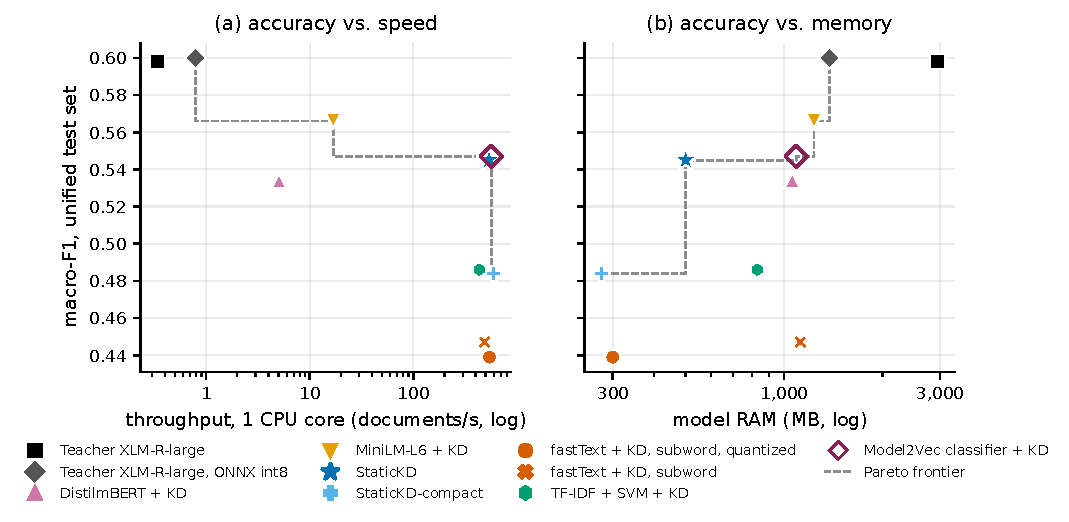
\includegraphics[width=0.85\textwidth]{figures/fig_tradeoff_memory.pdf}
\caption{Test macro-F1 against CPU throughput and RAM.}
\label{fig:tradeoff}
\end{figure*}
Table~\ref{tab:eff} shows that the teacher is too slow on CPU for a large stream of articles and that StaticKD removes this cost almost entirely. The PyTorch fp32 teacher needs 2,816~ms per article on one core and reaches a throughput of 0.34 articles per second. The best CPU configuration for the teacher is ONNX int8 (1,190~ms per article and 0.79 articles per second). These speeds mean that classifying one million articles per day would take 14.7 cores (ONNX int8) to 33.7 cores (PyTorch) for this step alone. The same load needs 0.02 cores with StaticKD.

The single-core speed of StaticKD exceeds that of every transformer-based model and is similar to that of the other light models. StaticKD needs 2.01~ms per article and can process 539 articles per second per core. This speed is about 682 times that of the ONNX int8 teacher and 1,572 times that of the PyTorch teacher. The distilled MiniLM-L6 and DistilmBERT are still about 32 and 107 times slower than StaticKD. The single-core speeds of the other light models range from 433 articles per second for TF-IDF + SVM to 601 for the compact variant. Tokenization limits the speed of StaticKD because it takes 98\% of the single-thread prediction time with 579 tokens per article on average whereas the averaging of table rows that follows tokenization reaches 26,843 articles per second when measured alone.

StaticKD also needs a smaller file than the teacher and a smaller file and less RAM than the Model2Vec classifier. The StaticKD file is 16 times smaller than that of the ONNX int8 teacher. The Model2Vec classifier that matches the accuracy of StaticKD needs 507~MB on disk and 1,091~MB of RAM compared with 501~MB of RAM for StaticKD. Fig.~\ref{fig:tradeoff} plots test macro-F1 against single-core throughput in panel (a) and RAM in panel (b) on log scales with the Pareto frontier as a dashed line. StaticKD and the Model2Vec classifier tie in panel (a) because their macro-F1 is equivalent and their throughputs over the three measurement sessions overlap (530--553 and 547--569 articles per second). The RAM of StaticKD is mostly taken by the tokenizer structure and falls to 277~MB in the compact variant. The quantized fastText + KD is smaller (18~MB) and uses less RAM (300~MB) than StaticKD but reaches a test macro-F1 of 0.439.

\subsection{Ablation, Temperature, and Ensembling}
\label{sec:res-abl}
\begin{table*}[!t]
\caption{Ablations and Temperatures for a Single Student Without Ensembling}
\label{tab:ablation}
\centering
\scriptsize
\begin{tabular}{@{}lccccc@{}}
\toprule
Variant & Seeds & Dev macro-F1 & Held-out agreement & Test macro-F1 & $\Delta$ test macro-F1 [95\% CI] \\
\midrule
\multicolumn{6}{@{}l}{\textit{Final recipe}} \\
\quad Final recipe (one seed) & 10 & 0.755$\pm$0.010 & 0.808$\pm$0.001 & 0.542$\pm$0.004 & -- \\
\multicolumn{6}{@{}l}{\textit{Component ablation}} \\
\quad Hard teacher labels (cross-entropy) & 5 & 0.749$\pm$0.007 & 0.805$\pm$0.001 & 0.547$\pm$0.004 & +0.005 [$-$0.002, +0.010]$^{\dagger}$ \\
\quad EMMediaTopic only (4 languages, 20k) & 5 & 0.723$\pm$0.006$^{*}$ & 0.730$\pm$0.001$^{*}$ & 0.491$\pm$0.002$^{*}$ & $-$0.051 [$-$0.064, $-$0.036] \\
\quad 130k documents (no extra CC-News) & 5 & 0.736$\pm$0.009$^{*}$ & 0.799$\pm$0.002$^{*}$ & 0.541$\pm$0.002 & $-$0.002 [$-$0.008, +0.002]$^{\dagger}$ \\
\quad Randomly initialized embedding & 5 & 0.715$\pm$0.005$^{*}$ & 0.739$\pm$0.004$^{*}$ & 0.422$\pm$0.006$^{*}$ & $-$0.120 [$-$0.166, $-$0.047] \\
\quad Frozen embedding (linear head only) & 5 & 0.720$\pm$0.001$^{*}$ & 0.788$\pm$0.001$^{*}$ & 0.557$\pm$0.002 & +0.014 [$-$0.004, +0.024] \\
\quad No token dropout & 5 & 0.757$\pm$0.004 & 0.808$\pm$0.001 & 0.544$\pm$0.002 & +0.001 [$-$0.001, +0.003]$^{\dagger}$ \\
\quad 512-unit MLP head (cannot be folded) & 5 & 0.762$\pm$0.009 & 0.813$\pm$0.002$^{*}$ & 0.551$\pm$0.006 & +0.009 [$-$0.000, +0.012] \\
\multicolumn{6}{@{}l}{\textit{Temperature}} \\
\quad $\tau=0.5$ & 5 & 0.750$\pm$0.004 & 0.807$\pm$0.002 & 0.546$\pm$0.005 & +0.004 [$-$0.002, +0.007]$^{\dagger}$ \\
\quad $\tau=2$ & 5 & 0.748$\pm$0.003 & 0.801$\pm$0.001$^{*}$ & 0.537$\pm$0.001 & $-$0.005 [$-$0.010, +0.008]$^{\dagger}$ \\
\quad $\tau=4$ & 5 & 0.723$\pm$0.004$^{*}$ & 0.791$\pm$0.001$^{*}$ & 0.529$\pm$0.002 & $-$0.014 [$-$0.020, +0.001] \\
\bottomrule
\end{tabular}
\par\vspace{2pt}{\footnotesize Mean $\pm$ standard deviation over seeds; $^{*}$ = different from the final recipe (paired bootstrap, Holm, $p<0.05$); $\Delta$ = test macro-F1 minus that of the final recipe [95\% CI]; $^{\dagger}$ = equivalent within $\pm$0.01 (TOST).\par}
\end{table*}
\begin{table}[!t]
\caption{Macro-F1 of Selected Variants by Distillation Data of the Article Language}
\label{tab:ablation-groups}
\centering
\footnotesize
\setlength{\tabcolsep}{3pt}
\resizebox{\columnwidth}{!}{%
\begin{tabular}{@{}lcccc@{}}
\toprule
Variant & Dev & Sufficient ($\ge$500) & Few ($<$500) & None (0) \\
\midrule
Final recipe (one seed) & 0.755 & 0.615 & 0.482 & 0.403 \\
Frozen embedding (linear head only) & 0.720 & 0.607 & 0.541 & 0.440 \\
Randomly initialized embedding & 0.715 & 0.567 & 0.182 & 0.161 \\
EMMediaTopic only (4 languages, 20k) & 0.723 & 0.559 & 0.466 & 0.351 \\
Hard teacher labels (cross-entropy) & 0.749 & 0.617 & 0.482 & 0.410 \\
512-unit MLP head (cannot be folded) & 0.762 & 0.613 & 0.484 & 0.421 \\
$\tau=2$ & 0.748 & 0.612 & 0.476 & 0.363 \\
\bottomrule
\end{tabular}}
\end{table}
\begin{figure}[!t]
\centering
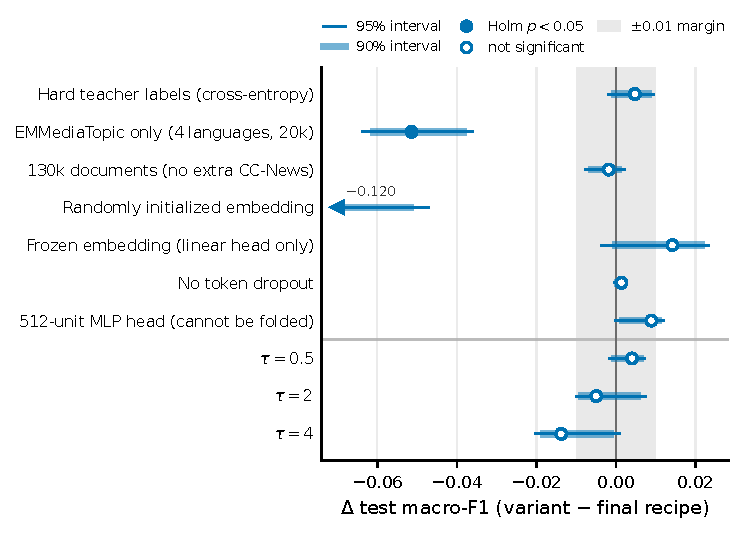
\includegraphics[width=\columnwidth]{figures/fig_ablation_forest.pdf}
\caption{Difference in test macro-F1 between each ablation variant and the final recipe.}
\label{fig:abl-forest}
\end{figure}
Table~\ref{tab:ablation} shows that most of the accuracy comes from two components: multilingual distillation data and the pre-trained embeddings. A student distilled on EMMediaTopic alone (4 languages) in place of the multilingual distillation data loses 0.051 in test macro-F1 and 0.077 in held-out agreement. Replacing the pre-trained potion embeddings with random initialization lowers the test macro-F1 more than any other variant (0.120, $p<0.001$). Fig.~\ref{fig:abl-forest} shows that only these two variants differ significantly from the final recipe in test macro-F1.

Freezing the embeddings restricts training to the linear head on top of potion and gives mixed results. The development score drops by 0.035 ($p=0.040$) and the held-out agreement by 0.020 ($p<0.001$). The test macro-F1 instead rises by 0.014 with an interval that includes zero ([$-$0.004, +0.024], $p=1.000$). Table~\ref{tab:ablation-groups} traces this gain to languages with little distillation data (+0.059) and to languages without distillation data (+0.037). The frozen embeddings score slightly lower in languages with at least 500 documents ($-$0.007).

None of the other variants changes the test macro-F1 significantly. Hard labels from the teacher raise the test macro-F1 by 0.005 ($p=1.000$) and lower the development score by 0.006 ($p=1.000$). The 90\% interval of the test difference lies inside the equivalence margin ([$-$0.001, +0.009], TOST $p=0.017$). This test shows that hard labels work as well as soft labels. Reducing the data to 130 thousand documents lowers the test score by 0.002 ($p=1.000$) and the held-out agreement by 0.009 ($p<0.001$) but its test difference still passes the equivalence test. Removing token dropout raises the test macro-F1 by 0.001 ($p=1.000$) and also passes the equivalence test. An MLP head that cannot be folded raises the test macro-F1 by 0.009 ($p=0.780$) but fails the equivalence test because its 90\% interval reaches +0.012.

A higher temperature does not help. The common choice of $\tau=2$~\cite{hinton2015distilling} lowers the held-out agreement by 0.007 ($p<0.001$) compared with $\tau=1$. The test macro-F1 and the development score do not change significantly at this setting ($-$0.005 and $-$0.006, both $p=1.000$). The test difference passes the equivalence test at both $\tau=2$ and $\tau=0.5$. The value $\tau=4$ lowers the development score and the held-out agreement significantly. Its drop of 0.014 in test macro-F1 is not significant ($p=0.836$).

A larger ensemble gives a small gain. Three seeds instead of one raise the test macro-F1 from 0.542 to 0.544 and the held-out agreement from 0.808 to 0.810. Ten seeds raise the test macro-F1 to 0.546. The gain comes at no cost at inference time because an ensemble of any size folds into one table.

\subsection{Analysis by Language, Label, Source, and Token}
\label{sec:res-lang}
Table~\ref{tab:groups} shows that the share of the teacher score that StaticKD keeps varies more with the amount of distillation data in the language of the article than with the label origin. The share by label origin ranges from 89.5\% for publisher categories to 95.8\% for JSON-LD sections. Grouping by distillation data shows a share that falls from 97.5\% in languages with at least 500 distillation documents to 72.3\% in languages without distillation data. This subgroup without distillation data is also the only subgroup in Table~\ref{tab:groups} where the Model2Vec classifier leads StaticKD by more than 0.011 (0.429 against 0.402).

\begin{table*}[!t]
\caption{Test Macro-F1 by Subgroup}
\label{tab:groups}
\centering
\scriptsize
\setlength{\tabcolsep}{3.5pt}
\begin{tabular}{@{}lrccccccccc@{}}
\toprule
Subgroup & $n$ & Teacher & DistilmBERT & MiniLM & \textbf{StaticKD} & Model2Vec & fastText (q) & TF-IDF+SVM & fastText GPT & \% teacher \\
\midrule
\multicolumn{11}{@{}l}{\textit{Label origin}} \\
\quad human annotation & 4,094 & 0.463 & 0.436 & 0.436 & 0.414 & 0.414 & 0.328 & 0.393 & 0.027 & 90\% \\
\quad publisher category & 2,600 & 0.702 & 0.498 & 0.674 & 0.629 & 0.632 & 0.300 & 0.330 & 0.063 & 90\% \\
\quad JSON-LD section & 6,050 & 0.651 & 0.629 & 0.634 & 0.624 & 0.618 & 0.582 & 0.609 & 0.136 & 96\% \\
\multicolumn{11}{@{}l}{\textit{Distillation data of the language}} \\
\quad sufficient ($\ge$500) & 7,644 & 0.633 & 0.617 & 0.616 & 0.618 & 0.611 & 0.575 & 0.593 & 0.116 & 98\% \\
\quad few ($<$500) & 2,243 & 0.537 & 0.344 & 0.496 & 0.478 & 0.475 & 0.195 & 0.227 & 0.037 & 89\% \\
\quad none (0) & 2,857 & 0.557 & 0.452 & 0.502 & 0.402 & 0.429 & 0.176 & 0.230 & 0.048 & 72\% \\
\multicolumn{11}{@{}l}{\textit{Region}} \\
\quad Africa & 3,044 & 0.697 & 0.532 & 0.576 & 0.542 & 0.550 & 0.325 & 0.408 & 0.085 & 78\% \\
\quad South Asia & 2,681 & 0.575 & 0.410 & 0.544 & 0.509 & 0.510 & 0.241 & 0.276 & 0.046 & 88\% \\
\quad East/Southeast Asia \& Middle East & 1,574 & 0.636 & 0.620 & 0.621 & 0.622 & 0.612 & 0.555 & 0.629 & 0.085 & 98\% \\
\quad Europe & 5,445 & 0.653 & 0.637 & 0.638 & 0.638 & 0.631 & 0.598 & 0.610 & 0.136 & 98\% \\
\multicolumn{11}{@{}l}{\textit{Teacher pre-training coverage}} \\
\quad outside XLM-R pre-training & 1,750 & 0.719 & 0.586 & 0.620 & 0.501 & 0.495 & 0.346 & 0.457 & 0.086 & 70\% \\
\quad in XLM-R pre-training & 10,994 & 0.609 & 0.549 & 0.585 & 0.576 & 0.572 & 0.471 & 0.503 & 0.096 & 95\% \\
\multicolumn{11}{@{}l}{\textit{Site diversity}} \\
\quad diverse ($\ge$10) & 5,225 & 0.657 & 0.642 & 0.643 & 0.642 & 0.637 & 0.601 & 0.616 & 0.134 & 98\% \\
\quad single publisher ($<$3) & 6,204 & 0.517 & 0.387 & 0.475 & 0.433 & 0.435 & 0.224 & 0.287 & 0.045 & 84\% \\
\quad medium (3--10) & 1,315 & 0.559 & 0.556 & 0.539 & 0.543 & 0.532 & 0.503 & 0.533 & 0.089 & 97\% \\
\bottomrule
\end{tabular}
\end{table*}

The share also differs by the source of the article. MN-DS is the only source annotated directly with IPTC topics and StaticKD keeps 97.4\% of the teacher score on this source (0.535 against 0.549). This high share is reached on the source where the macro-F1 of the teacher itself is lower than on any other source. The smallest share occurs on MasakhaNEWS (80.0\%) with its human labels following a non-IPTC scheme and 11 of its 16 languages absent from the distillation data.

The left panel of Fig.~\ref{fig:lang} shows that the accuracy gap between StaticKD and the teacher is small with a median of $-$0.024 per language. The gap narrows as the amount of distillation data grows ($\rho=0.52$, $p<0.001$). Held-out agreement with the teacher rises with teacher confidence ($\rho=0.71$, $p<0.001$) but its relation to the log amount of distillation data ($\rho=0.31$) is not significant after Holm correction ($p=0.067$). Agreement also does not differ significantly across scripts (Kruskal--Wallis $H=10.37$, $p=0.067$). The right panel of Fig.~\ref{fig:lang} shows that the held-out agreement of StaticKD is higher than that of the quantized fastText + KD in 52 of 53 languages.

The weak spot of StaticKD is a group of African languages. StaticKD reaches a mean accuracy of 0.407 on languages that lie outside XLM-R pre-training and are also absent from the distillation data (Igbo, Luganda, Lingala, Nigerian Pidgin, Kirundi, Shona, Tigrinya, and Yoruba). The teacher reaches 0.643 on the same languages. StaticKD is more accurate on Indian languages that are absent or nearly absent from the distillation data than on these African languages.

Four Indian languages (Bangla, Malayalam, Odia, and Punjabi) show how StaticKD behaves on text whose tokens hardly ever appeared in training. StaticKD reaches 0.748 on Bangla news even though this language is absent from the distillation data. Both fastText + KD and TF-IDF + SVM collapse on the same articles (0.191 and 0.010). At least 67\% of the token occurrences in these languages come from tokens that appear fewer than 10 times in the distillation data. StaticKD still reaches a mean accuracy of 0.624 on these languages compared with 0.738 for the teacher. The compact variant removes these rare tokens from the tokenizer and its accuracy on the four languages falls to 0.013. The accuracy of the two models in the other languages is 0.578 for the compact variant and 0.640 for the full StaticKD.

\begin{figure*}[!t]
\centering
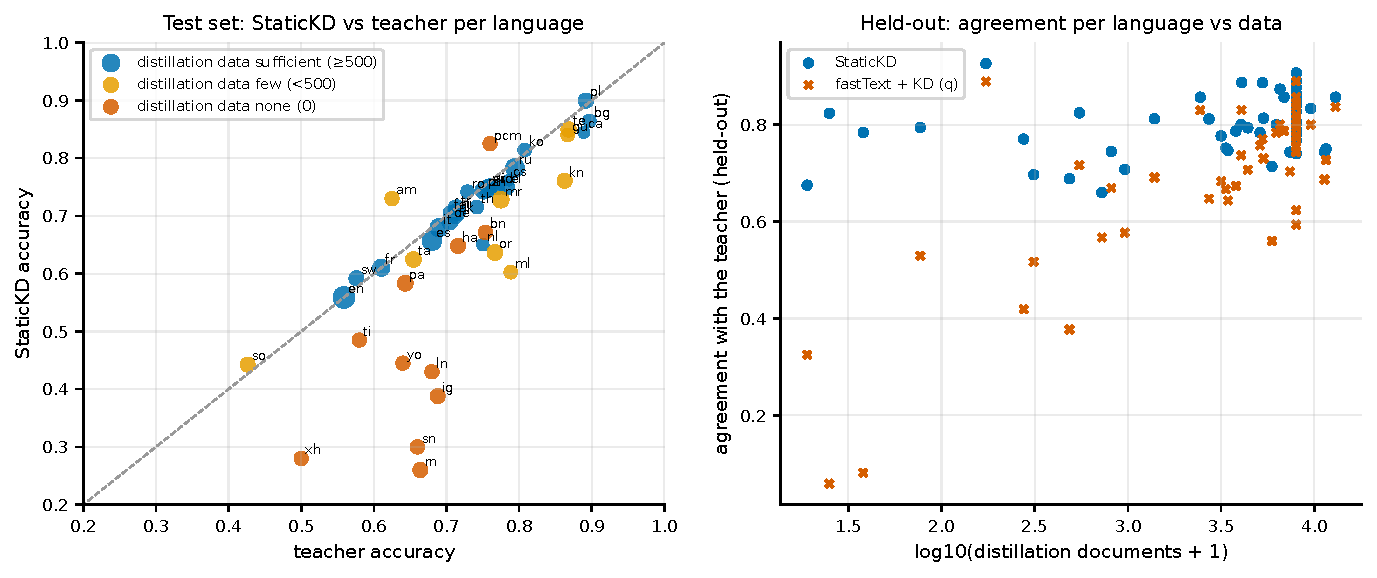
\includegraphics[width=0.8\textwidth]{figures/fig_per_language.pdf}
\caption{Per-language test accuracy of StaticKD against the teacher (left) and held-out agreement against distillation data (right).}
\label{fig:lang}
\end{figure*}

The performance of StaticKD differs across labels and its four hardest labels also rank among the hardest for the teacher. The StaticKD scores on these four labels are \emph{society} (0.16), \emph{disaster} (0.29), \emph{human interest} (0.32), and \emph{conflict} (0.37). The most frequent confusions are predictions of \emph{human interest} for \emph{society}, \emph{arts} for \emph{human interest}, and \emph{politics} for \emph{society} at 20\% each. StaticKD does best on \emph{sport} (0.88), \emph{weather} (0.84), and \emph{education} (0.75). The largest gaps to the teacher occur for \emph{environment} ($-$0.17), \emph{religion} ($-$0.15), and \emph{arts} ($-$0.08).

The token table of StaticKD also shows which tokens carry the topic signal of an article. Keeping only the 10\% most specific tokens of each article leaves the test macro-F1 almost unchanged (0.543 with about 58 tokens per article against 0.545 with all tokens). A random 10\% of the tokens gives only 0.435.

\subsection{Calibration and Cascade Mode}
\begin{table}[!t]
\caption{Cascade of StaticKD and the ONNX Int8 Teacher on the Test Set}
\label{tab:cascade}
\centering
\footnotesize
\setlength{\tabcolsep}{2.5pt}
\resizebox{\columnwidth}{!}{%
\begin{tabular}{@{}lccccc@{}}
\toprule
$\theta$ & StaticKD share & Accuracy on share & Macro-F1 & Accuracy & doc/s \\
\midrule
0 (StaticKD only) & 100.0\% & 0.641 & 0.545 & 0.641 & 539 \\
0.5 & 80.8\% & 0.732 & 0.586 & 0.690 & 4.09 \\
0.6 & 74.0\% & 0.760 & 0.593 & 0.697 & 3.02 \\
0.7 & 67.4\% & 0.788 & 0.600 & 0.702 & 2.41 \\
0.8 & 60.3\% & 0.813 & 0.602 & 0.703 & 1.98 \\
0.9 & 51.7\% & 0.839 & 0.602 & 0.703 & 1.63 \\
Teacher only & 0.0\% & -- & 0.600 & 0.699 & 0.79 \\
\bottomrule
\end{tabular}}
\end{table}
StaticKD is better calibrated than the teacher. The ECE of StaticKD is 0.041 on the development set and 0.139 on the test set against 0.090 and 0.245 for the teacher. Both models become overconfident on the out-of-distribution test set. The cascade mode uses this confidence to select the articles that StaticKD decides. Table~\ref{tab:cascade} shows that a higher threshold $\theta$ passes more articles to the teacher. The higher threshold raises the accuracy on the StaticKD share from 0.732 to 0.839 but lowers the effective throughput from 4.09 to 1.63 articles per second. The cascade at $\theta=0.8$ reaches an overall accuracy of 0.703 and a macro-F1 of 0.602 against 0.699 and 0.600 for the teacher alone. StaticKD itself decides 60.3\% of the articles in this cascade with an accuracy of 0.813. The effective throughput of this cascade is 1.98 articles per second per core and 2.5 times that of the teacher alone (0.79).

\section{Discussion}
\label{sec:discussion}
\subsection{Information Retained by the Token Table}
A table lookup keeps about nine tenths of the teacher macro-F1 and cuts inference time by about three orders of magnitude (Sections~\ref{sec:res-acc} and~\ref{sec:res-eff}). A table suffices because a small share of topic-specific tokens carries almost all of the topic signal in an article (Section~\ref{sec:res-lang}). The finding agrees with the observation of~\cite{galke2022bow} that order-free representations are already competitive for topic classification.

StaticKD scores lowest on \emph{society}, \emph{disaster}, \emph{human interest}, and \emph{conflict} but these low scores are not specific to the student. The same labels rank among the hardest for the teacher (Section~\ref{sec:res-lang}) and even human annotators find \emph{society} and \emph{human interest} difficult~\cite{kuzman2025llm}. The remaining gap to the teacher lies in other labels and in languages that are underrepresented in the distillation data (Section~\ref{sec:res-lang}).

\subsection{Sources of Accuracy}
The largest contribution comes from the pre-trained multilingual initialization and the second-largest from the multilingual distillation data labeled by the teacher. Random initialization costs 0.120 in test macro-F1 against 0.051 for removing the multilingual data. The most direct evidence for the role of the initialization comes from the compact variant on four Indian languages that hardly occur in the distillation data (Section~\ref{sec:res-lang}). Rare tokens in these languages keep embeddings close to the potion values because training rarely or never updates them. Accuracy in these languages is still close to that in other languages but falls almost to zero once the compact tokenizer removes these tokens. The drop reveals that transfer to languages without data relies on embeddings that training hardly changes. The linear head learned from data-rich languages still applies to such embeddings because the embeddings lie in the same space as the trained ones. Initialization also distinguishes StaticKD from Sparse Distillation~\cite{ye2022sparse} with its n-gram table trained from scratch. Pre-trained multilingual embeddings folded into 17 logits per token allow transfer to languages that are missing from the distillation data.

Freezing the embeddings raises the mean scores of languages with little or no distillation data (Table~\ref{tab:ablation-groups}). Fine-tuning moves the embeddings of tokens from the training languages whereas tokens from other languages stay at the positions assigned by potion. The head of the model has adapted to the moved embeddings and fits the unmoved tokens less well. This shift also fits the model better to the training languages. Frozen embeddings miss the shift and score lower on the development set. Fine-tuning and freezing may therefore trade fit to the training languages against the cross-lingual alignment inherited from potion. The final recipe uses fine-tuning because the development set on which it was selected is in the training languages and measures only the first side of this trade-off. Freezing gives no significant gain on the whole test set but is worth testing for a deployment that targets languages without distillation data.

The comparison of MiniLM-L6 and DistilmBERT as two transformer students also points to the role of the initial multilingual representation. The two models learn from the same distillation data and both have six layers but their initial representations differ because MiniLM comes from a distillation of XLM-R-large and DistilmBERT from mBERT. Only MiniLM-L6 closes part of the gap to the teacher (Table~\ref{tab:sig}).

StaticKD and the Model2Vec classifier likely owe their accuracy mainly to the shared embeddings and the teacher-labeled data rather than to the head. The Model2Vec classifier uses the same embeddings and data as StaticKD but learns from the top teacher label and adds a weight per token and a hidden layer (Table~\ref{tab:baselines}). It still reaches the same test macro-F1 as StaticKD within an equivalence margin of $\pm$0.01 that is less than half of the gap between StaticKD and MiniLM-L6 (Table~\ref{tab:sig}). The ablations in Section~\ref{sec:res-abl} also show no significant gain in test macro-F1 from the MLP head.

Soft labels add little or nothing. Hard teacher labels are equivalent to soft labels at $\tau=1$ within $\pm$0.01 macro-F1 and a higher temperature never improves on $\tau=1$ (Section~\ref{sec:res-abl}). The pattern fits the literature on the capacity gap~\cite{zhang2025law,wang2026rckd}. One linear layer over averaged embeddings may be unable to represent the inter-class structure in the tail of the teacher distribution (dark knowledge)~\cite{zhao2022dkd}. A high $\tau$ asks the student to imitate a distribution shape beyond its capacity.

Agreement with the teacher also does not always predict accuracy on independent labels and is therefore not enough to select a student~\cite{stanton2021kd}. Cutting the data to 130 thousand documents lowers the agreement significantly but leaves the test macro-F1 equivalent to that of the final recipe. The frozen-embedding variant scores lower in held-out agreement but higher in test macro-F1 although this gain is not significant (Section~\ref{sec:res-abl}). Student selection should therefore use labels that do not come from the teacher and a development set outside the training distribution.

\subsection{Weak Languages}
Per-language performance rises with how well a language is represented in the distillation data and the pre-training data. The weakest group consists of African languages outside XLM-R pre-training that are also absent from the distillation data (Section~\ref{sec:res-lang}). Subwords shared with other languages and sentence context may explain why the teacher stays more accurate than StaticKD on these languages. The cheapest fix requires no change of architecture because the teacher can label news in these languages to be added to the distillation data. The data ablation and the correlation between the accuracy gap and the amount of data ($\rho=0.52$) support adding such news.

\subsection{Practical Implications}
StaticKD suits a real-time pipeline on servers without a GPU and can be adjusted when a job demands higher accuracy or less RAM. The Model2Vec classifier and StaticKD run at a similar speed. StaticKD folds into one table so its file and RAM use are smaller and it needs only the \texttt{numpy} and \texttt{tokenizers} libraries (Table~\ref{tab:eff}). The output probabilities of StaticKD are better calibrated than those of the teacher and allow a cascade mode suited to batch jobs that need teacher-level accuracy. The compact variant of StaticKD lowers RAM but is advisable only when all target languages are already covered by the distillation data.

\subsection{Limitations}
\label{sec:limitations}
Test scores should be read with the nature of the labels in mind. An article about a criminal case that involves an athlete can rightly sit in a sports section whereas a model can label the same article \emph{crime}. Both answers are plausible because IPTC allows several topics per article. Comparisons between models remain fair because all models are scored against the same labels. The scope of this study is limited to single-label classification on top-level IPTC labels and leaves multi-topic articles and labels at deeper levels untested.

Section labels and publisher categories follow how publishers categorize articles and absolute scores on these labels therefore measure agreement with this categorization. Section conventions differ from one publisher to another and a section reflects one editorial view of an article that may cover several topics. This limitation of editorial labels holds especially for \emph{society}, \emph{human interest}, \emph{lifestyle}, and other labels with unclear boundaries.

Most test-set labels were not annotated directly with IPTC topics and their validity therefore depends on the mapping. Direct annotation with IPTC topics exists only in the English MN-DS dataset whereas the multilingual IPTC test set of Kuzman and Ljube\v{s}i\'c~\cite{kuzman2025llm} is not public. MasakhaNEWS labels also come from human annotators but follow a non-IPTC scheme and were then mapped to IPTC. Section labels were mapped with a conservatively built table that was validated against the IPTC tree and then evaluated and corrected manually but this manual evaluation produced no measure of agreement between reviewers.

Label coverage is uneven across languages. The median number of labels that occur in a language is 7 and the African languages cover only three to five broad topics. Per-language scores cannot be compared directly between languages with different label coverage because macro-F1 is computed over the labels present.

Site diversity is also limited. Twenty-seven languages have fewer than 3 effective sites. Articles in these languages come mostly from MasakhaNEWS, L3Cube-IndicNews, the Bangla news dataset, or one or two CC-NEWS sites. Claims about these languages hold only for those sources. The site-cluster bootstrap widens the confidence intervals of these languages accordingly. All test-set intervals rest on a small number of independent sources because the whole test set has an effective number of only 13.8 clusters.

The choice of baselines, the tuning budget, and the input length of the transformers limit the comparison of StaticKD with other models. Sparse Distillation~\cite{ye2022sparse} was not run as a baseline. It differs from fastText + KD and from the random-initialization ablation in the hidden layers of its deep averaging network, its soft-logit targets, and its billion-parameter n-gram table designed for English. Tuning budgets differed across models. The StaticKD recipe was fixed on the development set before the test set was built and the fastText and TF-IDF baselines were tuned on the same set with small grids. The Model2Vec classifier used the library defaults and the transformer models followed a standard fine-tuning recipe in which only $\tau$ of MiniLM-L6 was searched. MiniLM-L6 and DistilmBERT also read at most 256 tokens in the main comparison and therefore see less than half of the text of most test articles. Retraining both models with 512 tokens raises the test macro-F1 by 0.014 and 0.012 without changing the outcome of the comparison with StaticKD (Section~\ref{sec:res-acc}).

Efficiency measurements rest on one machine. The whole benchmark ran on one laptop (Section~\ref{sec:effprotocol}) and the latency of the teacher and the transformer models was measured on only 100 documents. Absolute numbers will differ on a server but ratios between models measured under the same protocol remain informative.

The weakness of StaticKD on African languages that are absent from both the distillation data and the pre-training data (Section~\ref{sec:res-lang}) means that a topic filter based on this model could misclassify or drop news in these languages more often. Accuracy should be monitored per language during deployment. Articles with low confidence should be routed to the teacher through the cascade mode.

The teacher bounds the performance of the student from above and passes its errors and biases to the student. These inherited errors stay invisible on the held-out set because this set measures agreement with the teacher and not correctness.

\section{Conclusion}
\label{sec:conclusion}
The open multilingual IPTC classifier needs 1.2 to 2.8 seconds per article on one CPU core. StaticKD distills this classifier into a table of 17 logits per token. The student that produces this table was initialized from multilingual static embeddings and then trained on 285,999 teacher-labeled articles in 69 languages. The evaluation uses 12,744 test articles in 47 languages whose labels do not come from the teacher. This test set can be reused to evaluate other IPTC classifiers.

StaticKD reaches a macro-F1 of 0.545 on this test set (91.1\% of the teacher score) and processes 539 articles per second per CPU core. This speed is about 682 times that of the ONNX int8 teacher. The 34-MB model also needs no deep learning library. The Model2Vec classifier trained on the same teacher labels is equivalent to StaticKD in test macro-F1 but has a file 15 times larger and needs twice the memory.

The ablations show that the accuracy of this small student comes mainly from multilingual distillation data and pre-trained multilingual embeddings whereas soft labels are no better than hard labels. Frozen embeddings lower the score on the development set but give higher mean scores in languages with little or no distillation data although the gain on the whole test set is not significant.

StaticKD is weakest on the labels \emph{society}, \emph{disaster}, \emph{human interest}, and \emph{conflict} and on languages that appear in neither the distillation data nor the pre-training data of the teacher. The weakness on these languages calls for extending the distillation data to the weak languages and especially to the African languages outside XLM-R pre-training. Fine-tuning could also use a regularizer that keeps the embeddings close to the pre-trained space. Such a regularizer might give in-distribution accuracy and cross-lingual transfer at the same time.

Further work can also lower the cost of StaticKD and extend its tasks and evaluation. A faster tokenizer such as a direct word-to-table lookup is the next source of speed because tokenization takes 98\% of the inference time of StaticKD. Vocabulary pruning to shrink the model has to keep the rare tokens that languages with little or no distillation data depend on. Other open problems are cheap non-linear heads with quantized embeddings, hierarchical classification down to IPTC level 2, multi-label classification, and human IPTC annotation of a multilingual sample of the test set.

\section*{Code, Model, and Data Availability}
The code for this study is available at \todo{GitHub URL and Zenodo DOI} and covers data collection, test-set construction, teacher labeling, training, evaluation, and benchmarking. A notebook in the same location reproduces every number, table, and figure in this paper. The section-to-IPTC mapping table is also released with the code. The StaticKD models are available at \todo{Hugging Face URL}. The test set is released with its reconstruction script as a manifest of article URLs or IDs, labels, label origins, and text hashes. Article texts are not redistributed because of publisher copyright and the licenses of the source datasets. EMMediaTopic is available from the CLARIN.SI repository~\cite{emmediatopic2025}. The licenses of the assets used and released in this study are listed with the code.

\section*{Acknowledgment}
The authors thank the Department of Informatics Engineering, Sepuluh Nopember Institute of Technology, for supporting this research. The authors used Claude Opus 5.5 (Anthropic) under their direction to explore design options for the method and to run the exploratory and final experiments. It also wrote the experiment code, processed data (including the first draft of the section-to-IPTC mapping table), and drafted parts of the manuscript text. The authors wrote and revised the manuscript themselves, reviewed and verified all code, data, and results, and take full responsibility for its content and claims.

\bibliographystyle{IEEEtran}
\bibliography{references}

\begin{IEEEbiographynophoto}{Obi Kastanya}
\todo{author biography}
\end{IEEEbiographynophoto}

\begin{IEEEbiographynophoto}{Ananta Dwi Prayoga Alwy}
\todo{author biography}
\end{IEEEbiographynophoto}

\begin{IEEEbiographynophoto}{Dwi Sunaryono}
\todo{author biography}
\end{IEEEbiographynophoto}

\EOD

\end{document}
